%% $Id: paper.tex 59236 2018-04-25 08:28:29Z cfrioux $
%% $HeadURL: https://svn.cs.uni-potsdam.de/svn/reposWV/Papers/ExpansionAlg/trunk/paper.tex $

\documentclass{new_tlp}

\usepackage[utf8]{inputenc}
\usepackage{microtype}
\usepackage{xparse,xifthen}
\usepackage{natbib}
\usepackage{amsmath,amssymb}
\let\proof\relax
\let\endproof\relax
\usepackage{amsthm}%,thmtools,environ}
\usepackage{url}
\usepackage{listings}
\usepackage[dvipsnames]{xcolor}
\usepackage{tikz}
\usepackage{slashbox}

\makeatletter
\let\O@argtabularcr\@argtabularcr
\def\O@xtabularcr{\@ifnextchar[\O@argtabularcr{\ifnum 0=`{\fi}\cr}}
\let\O@tabacol\@tabacol
\let\O@tabclassiv\@tabclassiv
\let\O@tabclassz\@tabclassz
\let\O@tabarray\@tabarray
\def\author@tabular{\authorsize\def\@halignto{}\@authortable}
\let\endauthor@tabular=\endtabular
\def\author@tabcrone{{\ifnum0=`}\fi\O@xtabularcr\affilsize\itshape
 \let\\=\author@tabcrtwo\ignorespaces}
\def\author@tabcrtwo{{\ifnum0=`}\fi\O@xtabularcr[-3\p@]\affilsize\itshape
 \let\\=\author@tabcrtwo\ignorespaces}
\def\@authortable{\leavevmode \hbox \bgroup $\let\@acol\O@tabacol
 \let\@classz\O@tabclassz \let\@classiv\O@tabclassiv
 \let\\=\author@tabcrone \ignorespaces \O@tabarray}
\makeatother


\usepackage{xcolor,colortbl}
\usepackage{xintexpr, xinttools}
\usepackage{caption}
%\usepackage{colortbl}

\lstset{numberbychapter=false,basicstyle=\ttfamily,captionpos=b,floatplacement=t}

\renewcommand{\topfraction}{1}
\renewcommand{\bottomfraction}{1}
\renewcommand{\textfraction}{0}

\newcommand{\review}[1]{{\textcolor{red}{#1}}}

% - rules etc --------------------------------------------------------------------
\newcommand{\naf}[1]{\ensuremath{{\sim}{#1}}}
\newcommand{\poslits}[1]{\ensuremath{#1^+}}
\newcommand{\neglits}[1]{\ensuremath{#1^-}}
\newcommand{\body}[1]{\ensuremath{B(#1)}} % {\ensuremath{\mathit{body}(#1)}}
\newcommand{\pbody}[1]{\poslits{\body{#1}}} % {\ensuremath{\mathit{body}^+(#1)}}
\newcommand{\nbody}[1]{\neglits{\body{#1}}} % {\ensuremath{\mathit{body}^-(#1)}}
\newcommand{\head}[1]{\ensuremath{h(#1)}} % {\ensuremath{\mathit{head}(#1)}}

\newcommand{\Tsign}{\ensuremath{\mathbf{T}}}
\newcommand{\Fsign}{\ensuremath{\mathbf{F}}}
\newcommand{\Tlit}[1]{\ensuremath{\Tsign #1}}
\newcommand{\Flit}[1]{\ensuremath{\Fsign #1}}
\newcommand{\Ass}{\ensuremath{\mathbf{A}}}
\newcommand{\DL}{\ensuremath{\mathit{DL}}}

\newcommand{\code}[1]{{\ttfamily #1}}
\newcommand{\codeClass}[2]{\code{#2}}

% - systems ----------------------------------------------------------------------
%
\newcommand{\sysfont}{\textit}
\newcommand{\acthex}{\sysfont{acthex}}
\newcommand{\asparagus}{\sysfont{asparagus}}
\newcommand{\aspic}{\sysfont{aspic}}
\newcommand{\aspmt}{\sysfont{aspmt}}
\newcommand{\asprin}{\sysfont{asprin}}
\newcommand{\assat}{\sysfont{assat}}
\newcommand{\berkmin}{\sysfont{berkmin}}
\newcommand{\claspD}{\sysfont{claspD}}
\newcommand{\claspar}{\sysfont{claspar}}
\newcommand{\claspfolio}{\sysfont{claspfolio}}
\newcommand{\clasp}{\sysfont{clasp}}
\newcommand{\clingcon}{\sysfont{clingcon}}
\newcommand{\clingo}{\sysfont{clingo}}
\newcommand{\cmodels}{\sysfont{cmodels}}
\newcommand{\coala}{\sysfont{coala}}
\newcommand{\dingo}{\sysfont{dingo}}
\newcommand{\dflat}{\sysfont{dflat}}
\newcommand{\dlvhex}{\sysfont{dlvhex}}
\newcommand{\dlv}{\sysfont{dlv}}
\newcommand{\ezcsp}{\sysfont{ezcsp}}
\newcommand{\ftolp}{\sysfont{f2lp}}
\newcommand{\gecode}{\sysfont{gecode}}
\newcommand{\gidl}{\sysfont{gidl}\xspace}
\newcommand{\gnt}{\sysfont{gnt}}
\newcommand{\gringo}{\sysfont{gringo}}
\newcommand{\iclingo}{\sysfont{iclingo}}
\newcommand{\idp}{\sysfont{idp}}
\newcommand{\inca}{\sysfont{inca}}
\newcommand{\jdlv}{\sysfont{jdlv}}
\newcommand{\lparse}{\sysfont{lparse}}
\newcommand{\lptodiff}{\sysfont{lp2diff}}
\newcommand{\lptosat}{\sysfont{lp2sat}}
\newcommand{\lctocasp}{\sysfont{lc2casp}}
\newcommand{\mchaff}{\sysfont{mchaff}}
\newcommand{\metasp}{\sysfont{metasp}}
\newcommand{\mingo}{\sysfont{mingo}}
\newcommand{\minisat}{\sysfont{minisat}}
\newcommand{\nomorepp}{\sysfont{nomore++}}
\newcommand{\oclingo}{\sysfont{oclingo}}
\newcommand{\piclasp}{\sysfont{piclasp}}
\newcommand{\picosat}{\sysfont{picosat}}
\newcommand{\plasp}{\sysfont{plasp}}
\newcommand{\quontroller}{\sysfont{quontroller}}
\newcommand{\rosoclingo}{\sysfont{rosoclingo}}
\newcommand{\sag}{\sysfont{sag}}
\newcommand{\satz}{\sysfont{satz}}
\newcommand{\siege}{\sysfont{siege}}
\newcommand{\smodelscc}{\sysfont{smodels$_{\!cc}$}}
\newcommand{\smodelsr}{\sysfont{smodels}$_r$}
\newcommand{\smodels}{\sysfont{smodels}}
\newcommand{\unclasp}{\sysfont{unclasp}}
\newcommand{\wasp}{\sysfont{wasp}}
\newcommand{\zchaff}{\sysfont{zchaff}}
\newcommand{\zzz}{\sysfont{z3}}

\newcommand{\theory}{\emph{Theory}}
\newcommand{\hybrid}{\sysfont{Hybrid}}

\newcommand{\aspif}{\sysfont{aspif}}

\newcommand{\python}{Python}
\newcommand{\lua}{Lua}
\newcommand{\cpp}{C++}
\newcommand{\C}{C}
\newcommand{\java}{Java}
\newcommand{\haskell}{Haskell}

\newacro{ILP}{Integer Linear Programming}
\newacro{SAT}{Boolean Satisfiability}
\newacro{ASP}{Answer Set Programming}
\newacro{DSE}{Design Space Exploration}
\newacro{ASPmT}{\ac{ASP} modulo Theories}
\newacro{MOEA}{multi-objective evolutionary algorithm}
\newacro{MOOP}{multi-objective optimization problem}
\newacro{QF--IDL}{qunatifier-free integer difference logic}

% - hacks ----------------------------------------------------------------------

\newcommand{\neghspace}{\!\!\!\!\!}

%%% Local Variables:
%%% mode: latex
%%% TeX-master: "paper"
%%% End:


\allowdisplaybreaks

\title{Hybrid Metabolic Network Completion}

\author[C.~Frioux, T.~Schaub, S.~Schellhorn, A.~Siegel, and P.~Wanko]{%
  Clémence Frioux
  \\
  Univ Rennes, Inria, CNRS, IRISA F-35000 Rennes, France
  \and
  Torsten Schaub%  orsten \thanks{Affiliated with the
                          %     School of Computing Science at
                          %     Simon Fraser University,
                          %     Burnaby, Canada,
                          %     and the
                          %     Institute for Integrated and Intelligent Systems
                          %     at
                          %     Griffith University,
                          %     Brisbane, Australia.}
  \\
  Inria, Rennes, France \ and \ Universit\"at Potsdam, Germany
  \and
  Sebastian Schellhorn
  \\
  Universit\"at Potsdam, Germany
  \and
  Anne Siegel
  \\
  Univ Rennes, Inria, CNRS, IRISA F-35000 Rennes, France
  \and
  Philipp Wanko
  \\
  Universit\"at Potsdam, Germany} %


\begin{document}

\maketitle
\begin{abstract}

Answer Set Programming (ASP) is an approach to declarative problem
solving, combining a rich yet simple modeling language with high
performance solving capacities.
%
We here develop an ASP-based approach to
\textit{Curriculum-Based Course Timetabling} (CB-CTT),
one of the most widely studied course timetabling problems.
The resulting {\asap} system reads a CB-CTT instance 
of a standard input format and converts it into a set of ASP facts.
In turn, these facts are combined with a first-order encoding for CB-CTT solving, 
which can subsequently be solved by any off-the-shelf ASP systems.
%
We establish the competitiveness of our approach by empirically
contrasting it to the best known bounds obtained so far via
dedicated implementations. 
%
Furthermore, we extend the {\asap} system to multi-objective course timetabling
and consider \textit{minimal perturbation problems}.
%
\keywords{Educational Timetabling \and Course Timetabling \and Answer
  Set Programming \and 
  Multi-objective Optimization \and 
  Minimal Perturbation Problems}
% \PACS{PACS code1 \and PACS code2 \and more}
% \subclass{MSC code1 \and MSC code2 \and more}
\end{abstract}

%%% Local Variables:
%%% mode: latex
%%% TeX-master: "paper"
%%% End:

\section{Introduction}\label{intro}

\textit{Educational timetabling}~\citep{%
DBLP:journals/eor/BurkeP02,%
Lewis2007:survey,%
DBLP:journals/air/Schaerf99}
is generally defined as the
task of assigning a number of events, such as lectures and examinations,
to a limited set of timeslots (and perhaps rooms), 
subject to a given set of hard and soft constraints.
Hard constraints must be strictly satisfied.
Soft constraints must not necessarily be satisfied but
the overall number of violations should be minimal.
%
The educational timetabling problems can be 
classified into three categories:
\textit{school timetabling},
\textit{examination timetabling}, and
\textit{course timetabling}.
In this paper, 
we focus on \textit{curriculum-based course timetabling} 
(CB-CTT;~\citep{Bettinelli2015}), 
one of the most studied course timetabling problems.
%as well as \textit{post-enrollment course timetabling}.

The CB-CTT problems have been used in the third track of 
the second international timetabling competition 
(ITC-2007;~\citep{%
  GasperoMS/ITC2007,%
  DBLP:journals/informs/McCollumSPMLPGQB10}).
%
A web portal\footnote{\texttt{http://tabu.diegm.uniud.it/ctt/}}
for CB-CTT has been actively maintained by the ITC-2007 organizers%
~\citep{DBLP:journals/anor/BonuttiCGS12}.
The web site provides necessary infrastructures for benchmarking
such as validators, data formats, problem instances,
solutions in different formulations (uploaded by researchers), 
and visualizers.
All problem instances on the web are based on
real data from various universities in Europe.
The best known bounds on the web have been obtained by 
state-of-the-art CB-CTT solving techniques
including the winner algorithm of ITC-2007:
metaheuristics-based algorithms~\citep{%
  DBLP:journals/heuristics/AbdullahTMM12,%
%  ClarkHL/PATAT2008,%
  DBLP:conf/patat/GasperoS02,%
  DBLP:journals/jmma/GasperoS06,%
  DBLP:journals/anor/Geiger12,%
  DBLP:journals/eor/LuH10},
Integer Programming~\citep{DBLP:journals/anor/LachL12},
hybrid methods~\citep{DBLP:journals/anor/Muller09},
SAT/MaxSAT~\citep{DBLP:journals/aicom/AchaN12},
and many others.

However, each method has strength and weakness.
Metaheuristics-based dedicated implementations can quickly find better
upper bounds, but cannot guarantee their optimality.
Although complete methods such as SAT can guarantee the optimality, 
it is costly to implement a dedicated encoder from the CB-CTT problems in SAT\@.
Integer Programming has been widely used for CB-CTT solving,
but in general it does not scale to large instances in complex formulations.
It is therefore particularly challenging to develop a universal
timetabling solver which can efficiently find optimal solutions 
as well as better bounds for a wide range of CB-CTT instances in
different formulations at present.

Answer Set Programming (ASP;~\citep{%
  baral03:cambridge,%
  DBLP:conf/iclp/GelfondL88,%
  DBLP:journals/amai/Niemela99})
is an approach to declarative problem solving.
Recent advances in ASP open up a successful direction to extend logic
programming to be both more expressive as well as more effective.
%
ASP provides a rich language and 
is well suited for modeling combinatorial (optimization) problems 
in Artificial Intelligence and Computer Science.
Recent remarkable improvements in the effectiveness of ASP systems
have encouraged researchers to use ASP for solving problems in diverse areas,
such as
automated planning,
constraint satisfaction,
model checking,
music composition,
robotics,
system biology,
etc~\citep{ergele16a}.
However, so far, little attention has been paid to using ASP for timetabling.

In this paper, we describe an ASP-based approach for solving the
CB-CTT problems and present the resulting {\asap} system.
The {\asap} system reads a CB-CTT instance 
of a standard input format~\citep{DBLP:journals/anor/BonuttiCGS12}
and converts it into ASP facts.
In turn, these facts are combined with a first-order encoding for
CB-CTT solving, which is subsequently solved by an off-the-shelf ASP
system, in our case {\clingo}.
% ~\footnote{%
% ASP system {\clingo} is a monolithic combination of the grounder {\gringo} with the solver {\clasp}.}.
Figure~\ref{fig:arch} shows the \asap\ architecture.
% ----------------------------------------------------------------------
\begin{figure}[t]
  \centering
%  \thicklines
  \setlength{\unitlength}{1.28pt}
  \small
  % \frame <- uncomment this to see the bounding box ;)
  {\begin{picture}(210,65)(4,-15)
    \put( 14, 20){\dashbox(26,24){\shortstack{CB-CTT\\Instance}}}
    \put( 50, 20){\framebox(40,24){\shortstack{Format\\Converter}}}
    \put(100, 20){\dashbox(20,24){\shortstack{ASP\\Facts}}}
    \put( 80,-10){\dashbox(40,24){\shortstack{ASP\\Encoding}}}
    \put(130, 20){\framebox(40,24){\clingo}}
    \put(180, 20){\dashbox(26,24){\shortstack{CB-CTT\\Solution}}}
    \put( 40, 32){\vector(1,0){10}}
    \put( 90, 32){\vector(1,0){10}}
    \put(120, 32){\vector(1,0){10}}
    \put(170, 32){\vector(1,0){10}}
    \put(120, +2){\line(1,0){4}}
    \put(124, +2){\line(0,1){30}}
  \end{picture}}
\caption{Architecture of \asap.}
\label{fig:arch}
\end{figure}
%%% Local Variables: 
%%% mode: latex
%%% TeX-master: "paper"
%%% End: 

% ----------------------------------------------------------------------

The high-level approach of ASP has obvious advantages.
First, the problems are solved by general-purpose ASP systems rather
than dedicated implementation.
Second,
the elaboration tolerance of ASP allows for easy maintenance and
modifications of encodings.
And finally,
it is easy to experiment with advanced techniques in ASP solving such
as core-guided optimization, domain heuristics, and 
portfolios of prefabricated expert configurations~\citep{gekakarosc15a}.
%
However, the question is whether the high-level approach of \asap\ matches the
performance of dedicated systems.
We empirically address this question by contrasting the performance of 
\asap\ with the best known bounds on the CB-CTT web portal
obtained by state-of-the-art CB-CTT solving techniques.

From the perspective of applying ASP to educational timetabling, 
an early work studied school timetabling with ASP~\citep{Faber98}.
Recently, we showed in previous work~\citep{basotainsc13a} that ASP's
modeling language is well-suited for course timetabling by providing
a compact encoding for CB-CTT solving.
However, at the same time, 
we observed that a simple branch-and-bound optimization strategy
is insufficient to decrease the upper bounds of large instances in complex formulations.
In this paper, we provide insights into how more advanced solving techniques can be used 
to overcome this practical issue.

The main contributions of this paper are as follows.
\begin{enumerate}
\item We present a basic ASP encoding for solving CB-CTT problems, 
  which is an enhancement of our previous encoding~\citep{basotainsc13a}. 
  This enhancement provides the ability to use advanced ASP solving
  techniques such as 
  core-guided optimization, 
  domain heuristics, 
  portfolios of prefabricated expert configurations,
  multi-criteria optimization based on lexicographic ordering, and
  multi-shot ASP solving~\citep{gekakarosc15a,gekaobsc15a}.
\item We extend the basic encoding in view of enhancing the
  scalability and flexibility of solving (multi-criteria) CB-CTT problems.
  The extended \asap\ encodings have the following features:
  \begin{itemize}
  \item A collection of optimized encodings for soft constraints
  \item Easy composition of different formulations
  \item Multi-criteria optimization based on lexicographic ordering
%  \item Reusing legacy timetables in multi-shot ASP solving
  \end{itemize}
\item Our empirical analysis considers all 61 instances in 5
  different formulations, which are publicly available from the CB-CTT
  portal ($61\times 5 = 305$ combinations in a total)~\footnote{As of July 20, 2017}.
  Overall, \asap\ managed to either improve or reproduce the best
  known bounds for 182 combinations (59.7\% in the total).
  In detail, \asap\ provided 54 better bounds, 
  16 new optima,
  and 128 same bounds, 
  35 of which were proven optimal for the first time.
  Furthermore,
  \asap\ was able to produce upper bounds for very large instances in
  the category \verb+erlangen+ with every formulation, and 24 of them
  were unsolvable before.
\item We also extend the {\asap} system to finding Pareto optimal solutions
  of multi-objective course timetabling and consider
  \textit{minimal perturbation problems}~\citep{%
    BartakMR03,MullerRB04,RudovaMM11,Phillips2016}
  by utilizing multi-shot ASP solving techniques~\citep{gekaobsc15a}.
\end{enumerate}
All in all, the proposed declarative approach represents a significant
contribution to the state-of-the-art for CB-CTT.

The rest of the paper is structured as follows.
Section~\ref{sec:cb-ctt} provides the problem description of CB-CTT\@.
Although we give a brief introduction to ASP and its basic language
constructs in Section~\ref{sec:asp}, 
we refer the reader to the literature~\citep{baral03:cambridge,gekakasc12a}
for a comprehensive treatment of ASP\@.
Section~\ref{sec:approach}
describes {\asap}'s fact format of CB-CTT instances and then 
presents a basic {\asap} encoding for solving CB-CTT problems.
Section~\ref{sec:ext} presents a variety of features of
extended {\asap} encodings for (multi-criteria) CB-CTT solving.
Section~\ref{system} provides a detailed empirical analysis of {\asap}
features and performance in contrast to 
the best known bounds obtained by state-of-the-art CB-CTT solving techniques.
Section~\ref{mpp} presents an extension of the {\asap} system to 
minimal perturbation problems in course timetabling. 
Finally, a conclusion is given in Section~\ref{conclusion}.

%%% Local Variables:
%%% mode: latex
%%% TeX-master: "paper"
%%% End:

%!TEX root = paper.tex

\section{Metabolic Network Completion}\label{sec:problem}

Metabolism is the sum of all chemical reactions occurring within an organism.
As the products of a reaction may be reused as reactants, reactions can be chained to complex chemical pathways.
Such complex pathways are described by a metabolic network.

We represent a \emph{metabolic network} as a labeled directed bipartite graph
\(
G=(R\cup M,E,\StoichiometricFunction),
\)
where $R$ and $M$ are sets of nodes standing for \emph{reactions} and \emph{compounds} (also called metabolites), respectively.
%
When $(m,r)\in E$ or $(r,m)\in E$ for $m\in M$ and $r\in R$, the metabolite $m$ is called a \emph{reactant} or \emph{product} of reaction~$r$, respectively. \review{Metabolites and reactions nodes can both have multiple ingoing and outgoing edges.}
%
More formally, for any $r\in R$, define
\(
\Reactants{r}=\{m\in M\mid (m,r)\in E\}
\)
and
\(
\Products{r} =\{m\in M\mid (r,m)\in E\}
\).
%
%
The \emph{edge labeling}
\(
\StoichiometricFunction: E\rightarrow \mathbb{R}
\)
gives the stoichiometric coefficients of a reaction's reactants and products, respectively, i.e., their relative quantities involved in the reaction.
%
Finally, the activity rate of reactions is bound by lower and upper bounds,
denoted by $\MinFlux{r}\in\mathbb{R}^+_0$ and $\MaxFlux{r}\in\mathbb{R}^+_0$ for $r\in R$, respectively.
%
Whenever clear from the context,
we refer to metabolic networks with $G$ (or $G'$, etc) and denote the associated reactions and compounds with
$M$ and $R$ (or $M',R'$ etc), respectively.

We distinguish a set $S \subseteq M$ of compounds as initiation \emph{seeds}, that is,
compounds initially present due to experimental evidence.
%
Another set of compounds is assumed to be activated by default.
These \emph{boundary compounds} are defined as:
\(
\strseed(G) = \{ m\in M \mid r\in R,  m\in \Products{r}, \Reactants{r}=\emptyset \}
\).
%
For simplicity, we assume that all boundary compounds are seeds: $\strseed(G)\subseteq S$.
Note that follow-up concepts like reachability and activity in network completion are independent of this assumption.

For illustration, consider the metabolic network in Fig.~\ref{gra:toy_d}.
%
% ----------------------------------------------------------------------
\begin{figure}[t]
  \centering
    \input{toypic_draft}
    \caption{Example of a metabolic network. Compounds and reactions are depicted by circles and rectangles respectively. Dashed reactions are reactions involving the boundary between the organism's metabolism and its environment. $r_5$ is the target reaction. $S_1$ and $S_2$ are boundary (and initiation) seeds. $S_3$ is assumed to be an initiation seed. Numbers on arrows describe the stoichiometry of reaction (default value is 1).}
    \label{gra:toy_d}
\end{figure}
% ----------------------------------------------------------------------
%
The network consists of 9 reactions, \SeedReaction, \SeedReactiont, \ExportReaction{} and $r_0$ to $r_5$, and 8 compounds, $A,\dots,F$, $S_1$, $S_2$ and $S_3$.
Here, $S=\{S_1,S_2,S_3\}$, $S_1$ and $S_2$ being the two boundary compounds of the network. Dashed rectangle describes the boundary of the system, outside of which is the environment of the organism.
%
Consider reaction
\(
r_4 : E\rightarrow 2C
\)
transforming one unit of $E$ into two units of $C$ (stoichiometric coefficients of 1 are omitted in the graphical representation; cf.~Fig.~\ref{gra:toy_d}).
%
We have
$\Reactants{r_4}=\{E\}$,
$\Products{r_4}=\{C\}$,
along with $\Stoichiometry{E}{r_4}=1 $
\ and $\Stoichiometry{r_4}{C}=2$.

In biology, several concepts have been introduced to model the activation of reaction fluxes in metabolic networks,
or to synthesize metabolic compounds.
%
To model this,
we introduce a function \ActivityFunction\ that given a metabolic network $G$ takes a set of seeds $S \subseteq M$ and returns a set of activated
reactions $\Activitytwo{G}{S} \subseteq R$.
%
%
% ----------------------------------------------------------------------
\begin{figure}[t]
  \centering
    \input{toypic}
    \caption{Metabolic network completion problem. The purpose of its solving is to select the minimal number of reactions from a database (dashed shaded reactions) such that activation of target reaction $r_5$ is restored from boundary and/or initiation seeds. There are three formalisms for activation of target reaction: stoichiometric, topological and hybrid.}
    \label{gra:toy}
\end{figure}
% ----------------------------------------------------------------------
%
With it,
\emph{metabolic network completion} is about ensuring that a set of target reactions (reaction $r_5$ in~Fig.~\ref{gra:toy_d}) is activated from seed compounds in $S$
by possibly extending the metabolic network with reactions from a reference network (cf.\ shaded part in~Fig.~\ref{gra:toy}).

Formally, given
a metabolic network $G=(R\cup M,E,\StoichiometricFunction)$, % with bounds,
a set $S\subseteq M$ of seed compounds such that $\strseed(G) \subseteq S$,
a set $R_{T}\subseteq R$ of target reactions, and
a reference network $(R'\cup M',E',\StoichiometricFunction')$,
%
the \emph{metabolic network completion problem} is to find a set $R''\subseteq R'\setminus R$ of reactions of minimal size such that
\(
R_{T}\subseteq\Activitytwo{G''}{S}
\)
where%
\footnote{Since \StoichiometricFunction, $\StoichiometricFunction'$ have disjoint domains we view them as relations and compose them by union.}
\begin{align}
  \label{eq:completion:graph}
  G''&= ((R\cup R'')\cup (M\cup M''),E\cup E'',\StoichiometricFunction'')\ ,
  \\\label{eq:completion:metabolites}
  M''&=\{m\in M'\mid r\in R'', m\in\Reactants{r}\cup\Products{r}\}\ ,
  \\\label{eq:completion:edges}
  E''&=E'\cap((M''\times R'')\cup(R''\times M'')) , \text{ and}
  \\
  \StoichiometricFunction''&=\StoichiometricFunction\cup\StoichiometricFunction'
  \ .
\end{align}
%
We call $R''$ a \emph{completion} of $(R\cup M,E,\StoichiometricFunction)$ from $(R'\cup M',E',\StoichiometricFunction')$ wrt $S$ and $R_{T}$.
%
Our concept of activation allows different biological paradigms to be captured.
%
Accordingly,
different formulations of metabolic network completion can be characterized:
the stoichiometric, the relaxed stoichiometric, the topological, and the hybrid one.
We elaborate upon their formal characterizations in the following sections.

\subsection{Stoichiometric Metabolic Network Completion}\label{sec:stoichio} %\emph
%
The first activation semantics has been introduced in the context of Flux Balance Analysis
capturing reaction flux distributions of metabolic networks at steady state.
%
In this paradigm, each reaction $r$ is associated with a \emph{metabolic flux value},
expressed as a real variable $v_r$ confined by the minimum and maximum rates:
%
\begin{align} \label{eq:stoichiometric:bounds}
  & \MinFlux{r} \leq  v_r\leq \MaxFlux{r} \qquad\text{ for } r\in R.
\end{align}
%
Flux distributions are formalized in terms of a system of equations relying on the stoichiometric coefficients of reactions.
%
\review{Reaction stoichiometries are governed by the \emph{law of mass conservation} under a steady state assumption; in other words, the mass of the system remains constant over the reaction.
The input and output fluxes of reactions consuming and producing a metabolite are balanced.}
%
\begin{align}
\label{eq:stoichiometric:equation}
  & \textstyle
    \sum_{\substack{r\in R}}\Stoichiometry{r}{m}\cdot v_r
    +
    \sum_{\substack{r\in R}}-\Stoichiometry{m}{r}\cdot v_r
    =
    0
    \qquad \text{ for } m\in M.
\end{align}
%
Given a target reaction $r_T\in R_T$, a metabolic network $G=(R\cup M,E,\StoichiometricFunction)$ and a set of seeds $S$,
\emph{stoichiometric activation} is defined as follows:
\begin{align}%*
\label{eq:stoichiometric:activation}
  r_T \in \Activity{s}{G}{S} & \ \text{ iff } \ v_{r_T} >0 \text{ and }
                               \eqref{eq:stoichiometric:bounds} \text{ and } \eqref{eq:stoichiometric:equation}\text{ hold for }M\text{ and }R.
\end{align}%*
Note that the condition $v_{r_T} >0$ strengthens the flux condition for $r_T\in R$ in the second part.
More generally, observe that activated target reactions are not directly related to the network's seeds $S$.
However,
the activation of targets highly depends on the boundary compounds in $\strseed(G)$
for which \eqref{eq:stoichiometric:equation} \review{is always satisfied and thus initiates the fluxes.
Since boundary compounds are produced by at least one reaction without prerequisite,
an arbitrary amount might be produced.
Therefore, the incoming flux value always balances the sum of the flux values associated to outgoing edges.
Intuitively, boundary compounds are nutrients that are expected to be available in the system
for the consumption by the metabolic network,
thus initiating the reactions within.}
%
In our draft network $G$,
consisting of all \review{non-dashed} nodes and edges depicted in Fig.~\ref{gra:toy}
(viz.\ reactions \SeedReaction, \SeedReactiont, \ExportReaction{} and $r_0$ to $r_5$ and compounds $A,\dots,F$, $S_1$, $S_2$, and $S_3$ and $r_5$ the single target reaction)
and the reference network $G'$,
consisting of the shaded part of Fig~\ref{gra:toy},
(viz.\ reactions $r_6$ to $r_9$ and metabolite $G$)
a strict stoichiometry-based completion aims to obtain a solution with $r_5\in\Activity{s}{G''}{\{S_1,S_2,S_3\}}$ where $v_{r_5}$ is maximal.
%
This can be achieved by adding the completion $R''_1=\{r_{6},r_9\}$ (Fig.~\ref{gra:toy_ss}).
%
\review{The cycle made of compounds $E,C,D$ and the boundary seed $S_2$ is already balanced and notably self-activated.
Indeed, initiation of $D$ and $E$ producibility requires the producibility of $C$ (in addition to the presence of the boundary seed $S_2$) that itself depends on $D$ and $E$. Yet, according the flux conditions, that models steady state conditions, the cycle is activated.
Such self-activation of cyclic pathways is an inherent problem of purely stoichiometric approaches to network completion.
This is a drawback of the semantics because the effective activation of the cycle requires the additional (and unchecked) condition that at least one of the compounds was present as the initial state of the system. This could be the case provided there exist another way to enable the production of one or several components of the cycle (here an activable reaction producing $E$ for instance) \citep{Prigent2017}.}
%
The instance of Equation~\eqref{eq:stoichiometric:equation} controlling the reaction rates related to metabolite $C$ is
\(
2\cdot v_{r_4} - v_{r_2} - v_{r_5} = 0
\).


To solve metabolic network completion with flux-balance activated reactions,
Linear Programming can be used to maximize the flux rate $v_{r_T}$ provided that the linear constraints are satisfied.
%
Nonetheless, this problem turns out to be hard to solve in practice and existing approaches scale poorly to real-life applications (cf.~ \citep{Orth2010}).

This motivated the use of approximate methods.
%
The relaxed problem is obtained by weakening the mass-balance equation \eqref{eq:stoichiometric:equation} as follows:
%
\begin{align}
\label{eq:stoichiometric:equation:relaxed}
  &  \textstyle        \sum_{\substack{r\in R}} \Stoichiometry{r}{m}\cdot v_r
                       +
                       \sum_{\substack{r\in R}}-\Stoichiometry{m}{r}\cdot v_r
                       \geq
                       0
                       \qquad \text{ for } m\in M.
\end{align}
%
This lets us define the concept of \emph{relaxed stoichiometric activation}:
\begin{align}%*
\label{eq:stoichiometric:activation:relaxed}
  r_T \in \Activity{r}{G}{S} & \ \text{ iff } \ v_{r_T} >0 \text{ and }
                               \eqref{eq:stoichiometric:bounds} \text{ and } \eqref{eq:stoichiometric:equation:relaxed}\text{ hold for }M\text{ and }R.
\end{align}%*
The resulting problem can now be efficiently solved with Linear Programming~\citep{SatishKumar2007}.
%
Existing systems addressing strict stoichiometric network completion either
cannot guarantee optimal solutions~\citep{laten2014a} or
do not support a focus on specific target reactions~\citep{Thiele2014}.
Other approaches either partially relax the problem~\citep{Vitkin2012} or
solve the relaxed problem based on Equation~\eqref{eq:stoichiometric:equation:relaxed},
like the popular system \gapfill~\citep{SatishKumar2007}. Applied to the network of Fig.~\ref{gra:toy}, the minimal completion under the relaxed stoichiometric activation is $R''_1=\{r_{6}\}$  (Fig.~\ref{gra:toy_sr}) but does not carry flux because of the accumulation of metabolite $G$, allowed by Equation~\eqref{eq:stoichiometric:equation:relaxed}.
%
Note however that for strict steady-state modeling an \textit{a posteriori} verification of solutions is needed
to warrant the exact mass-balance equation~\eqref{eq:stoichiometric:equation}.


% ----------------------------------------------------------------------
\begin{figure}
    \captionsetup{width=0.45\textwidth}
    \centering
    \begin{minipage}[t]{.5\textwidth}
      \centering
      \input{toypic_sol_s}
      \caption{Solution to metabolic network completion under stoichiometric activation hypothesis in order to satisfy Equations~\eqref{eq:stoichiometric:bounds},~\eqref{eq:stoichiometric:equation} and ~\eqref{eq:stoichiometric:activation}. Within this network, there exists at least one flux distribution which activates $r_5$.}
      \label{gra:toy_ss}
    \end{minipage}%
    \begin{minipage}[t]{.5\textwidth}
      \centering
      %!TEX root = paper.tex
\usetikzlibrary{shapes.misc, positioning}
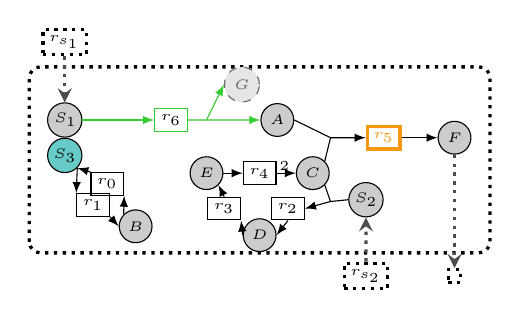
\begin{tikzpicture}[scale=0.45]\tiny
  \tikzstyle{metabolite}=[draw,circle,fill=white!80!black, text width=0.4cm, inner sep=0pt, align=center];
  \tikzstyle{repairmetabolite}=[draw,white!40!black, circle,fill=white!90!black,text=white!40!black,dashed];
  \tikzstyle{seed}=[draw,circle,fill=BlueGreen!70, text width=0.4cm, inner sep=0pt, align=center];%white!80!black
  \tikzstyle{target}=[draw,circle,fill=YellowOrange];%white!40!black
  \tikzstyle{reaction}=[draw,rectangle];
   \tikzstyle{export}=[draw,rectangle,dotted, very thick];
   \tikzstyle{exportrepair}=[draw,rectangle,dotted, very thick,white!80!black,text=white!70!black];
  \tikzstyle{repairreaction}=[draw,rectangle,white!40!black,text=white!40!black,dashed];
  \tikzstyle{solreaction}=[draw,rectangle,LimeGreen,text=black];
  \tikzstyle{initial}=[->,>=latex,thick];
  \tikzstyle{bdd}=[->,>=latex,thick];
  \tikzstyle{etiq}=[midway,fill=black!20,scale=0.5];
  \tikzstyle{stc}=[draw, rectangle, white, text=black]

  \node[stc] (stcr4C) at (6.2,6.7) {$2$};

  \draw [black,dotted, rounded corners, very thick] (-1,4.25) rectangle (12,9.5);
 % \node (system) [draw, rounded rectangle] at (0,0) {} (7cm,5cm);

  \node[seed] (S2) at (0,7) {$S_{3}$};
  \node[metabolite] (Sb2) at (8.5,5.75) {$S_{2}$};
  \node[metabolite] (S1) at (0,8) {$S_{1}$};

  \node[metabolite] (F) at (11,7.50) {$F$};

  \node[metabolite] (A) at (6,8) {$A$};
  \node[metabolite] (B) at (2,5.0) {$B$};
  \node[metabolite] (C) at (7,6.5) {$C$};
  \node[metabolite] (D) at (5.50,4.75) {$D$};
  \node[metabolite] (E) at (4,6.5) {$E$};
  \node[repairmetabolite] (X) at (5,9) {$G$};

  \node[reaction] (R0) at (1.2,6.2) {$r_{0}$};
  \node[reaction] (R1) at (0.8,5.60) {$r_{1}$};
  \node[reaction] (R2) at (6.3,5.5) {$r_{2}$};
  \node[reaction] (R3) at (4.5,5.5) {$r_{3}$};
  \node[reaction] (R4) at (5.5,6.5) {$r_{4}$};
  \node[reaction, very thick,YellowOrange] (R5) at (9,7.50) {$r_{5}$}; %LimeGreen
  \node[solreaction] (R6) at (3,8) {$r_{6}$};
  % \node[repairreaction] (R7) at (2.3,6.9) {$r_{7}$};
  % \node[repairreaction] (R8) at (3,5.8) {$r_{8}$};
  % \node[repairreaction] (R9) at (8.5,8.5) {$r_{9}$};

  % R0 : S => B
  \draw[->,>=latex] (B.north west) -- (R0.south east);
  \draw[->,>=latex] (R0.north west) -- (S2.south east);

  % R1 : S <= B
  \draw[->,>=latex] (S2.south east) -- (R1.north west);
  \draw[->,>=latex] (R1.south east) -- (B.west);

  % R2 : Sb2+C => D
  \draw[->,>=latex] (Sb2.west) -- (7.5,5.70) -- (R2.east);
  \draw[] (C.south east) -- (7.5,5.70);
  \draw[->,>=latex] (R2.south) -- (D.east);

  % R3 : D => E
  \draw[->,>=latex] (D.west) -- (R3.south east);
  \draw[->,>=latex] (R3.north) -- (E.south east);

  % R4 : E => C
  \draw[->,>=latex] (E.east) -- (R4.west);
  \draw[->,>=latex] (R4.east) -- (C.west);

  % R5 : A+C => T
  \draw[->,>=latex] (A.east) -- (7.5,7.50) -- (R5.west);
  \draw[] (C.north east) -- (7.5,7.50);
  \draw[->,>=latex] (R5.east) -- (F.west);

  % R6 : S => A+X
  \draw[->,>=latex,LimeGreen] (S1.east) -- (R6.west);
  \draw[->,>=latex,LimeGreen] (R6.east) -- (4,8) -- (A.west);
  \draw[->,>=latex,LimeGreen] (4,8) -- (X.west);

  % % R7 : S => E
  % \draw[->,>=latex,white!55!black,dashed] (S2.east) -- (R7.west);
  % \draw[->,>=latex,white!55!black,dashed] (R7.east) -- (E.north west);
  %
  % % R8 : B => E
  % \draw[->,>=latex,white!55!black,dashed] (B.north east) -- (R8.south west);
  % \draw[->,>=latex,white!55!black,dashed] (R8.east) -- (E.south);

  % % R9 : X => F
  % \draw[->,>=latex,green] (X.east) -- (R9.north west);
  % \draw[->,>=latex,green] (R9.east) -- (F.north west);

  %export X
  %\node[exportrepair] (outX) at (6.5,10.30) {$r_{expX}$};
  %\draw[->,>=stealth,white!80!black,dotted, very thick] (X.north east) --  (outX.west);

  %export F
  \node[export] (outF) at (11,3.6) {\ExportReaction};
   \draw[->,>=stealth,white!30!black,dotted, very thick] (F.south) --  (outF.north);

  %import S2
   \node[export] (inS) at (0,10.2) {$r_{s_1}$};
   \draw[->,>=stealth,white!30!black,dotted, very thick] (inS.south) --  (S1.north);

   %import Sb2
  \node[export] (inS2) at (8.5,3.6) {$r_{s_2}$};
  \draw[->,>=stealth,white!30!black,dotted, very thick] (inS2) --  (Sb2.south);

\end{tikzpicture}
%
%%% Local Variables:
%%% mode: latex
%%% TeX-master: "paper"
%%% End:

      \caption{Solution to metabolic network completion under relaxed stoichiometric activation hypothesis in order to satisfy Equations~\eqref{eq:stoichiometric:bounds},~\eqref{eq:stoichiometric:equation:relaxed} and ~\eqref{eq:stoichiometric:activation:relaxed}. Notice that within this completed network, there exist no flux distribution allowing the reaction $r_5$ to be activated.}
      \label{gra:toy_sr}
    \end{minipage}
\end{figure}
% ----------------------------------------------------------------------

\subsection{Topological Metabolic Network Completion}\label{sec:topo} %emph
%
A qualitative approach to metabolic network completion relies on the topology of networks for capturing the activation of reactions.
%
Given a metabolic network $G$, a reaction $r\in R$ is \emph{activated} from a set of seeds $S$ if all reactants in $\Reactants{r}$ are reachable from~$S$.
%
Moreover, a metabolite $m\in M$ is \emph{reachable} from $S$ if %
$m\in S$
or if
$m\in\Products{r}$ for some reaction $r\in R$ where all $m'\in\Reactants{r}$ are reachable from~$S$.
%
The \emph{scope} of $S$, written $\Sigma_G(S)$, is the closure of compounds reachable from~$S$.
%
In this setting, \emph{topological activation} of reactions from a set of seeds $S$ is defined as follows:
%
\begin{align}%*
  r_T \in \Activity{t}{G}{S} \ \text{ iff } \ \Reactants{r_T} \subseteq \Sigma_G(S).   \label{eq:topological:activation}
\end{align} %*
%
Note that this semantics avoids self-activated cycles by imposing an external entry sufficient to initiate all cycles ($S_3$ is not enough to activate the cycle as it does not activate one of its reaction on its own).
The resulting network completion problem can be expressed as a combinatorial optimization problem and effectively solved with ASP~\citep{schthi09a}.

For illustration, consider again the draft and reference networks $G$ and $G'$ in Fig.~\ref{gra:toy_d} and Fig.~\ref{gra:toy}.
%
We get $\Sigma_{G}(\{S_1,S_2,S_3\})=\{S_1,S_2,S_3,B\}$, indicating that target reaction $r_5$ is not activated from the seeds with the draft network
because $A$ and $C$, its reactants, are not reachable.
%
This changes once the network is completed.
%
Valid minimal completions are $R''_2=\{r_6,r_7\}$ (Fig.~\ref{gra:toy_st1}) and $R''_3=\{r_6,r_8\}$ (Fig.~\ref{gra:toy_st2}) because
\(
r_5\in\Activity{t}{G''_i}{\{S_1,S_2\}}\mbox{ since }\{A,C\}\subseteq\Sigma_{G''_i}(\{S_1,S_2\})
\)
for all extended networks $G''_i$ obtained from completions $R''_i$ of $G$ for $i\in\{2,3\}$.
%
% ----------------------------------------------------------------------
\begin{figure}
    \captionsetup{width=0.45\textwidth}
    \centering
    \begin{minipage}[t]{.5\textwidth}
      \centering
      \input{toypic_sol_t1}
      \caption{First solution to metabolic network completion under topological activation hypothesis satisfying Equation~\eqref{eq:topological:activation}. The production of C cannot be explained by a self-activated cycle and requires an external source of compounds via $S_3$ and reaction $r_7$.}
      \label{gra:toy_st1}
    \end{minipage}%
    \begin{minipage}[t]{.5\textwidth}
      \centering
      \input{toypic_sol_t2}
      \caption{Second solution to metabolic network completion under topological activation hypothesis satisfying Equation~\eqref{eq:topological:activation}.}
      \label{gra:toy_st2}
    \end{minipage}
\end{figure}
% ----------------------------------------------------------------------

Relevant elements from the reference network are given in dashed gray.

\subsection{Hybrid Metabolic Network Completion}\label{sec:hybrid} %emph
%
The idea of hybrid metabolic network completion is to combine the two previous activation semantics:
the topological one accounts for a well-founded initiation of the system from the seeds
and the stoichiometric one warrants its mass-balance.
%
We thus aim at network completions that are both topologically functional and flux balanced
(without suffering from self-activated cycles).
%
More precisely,
a reaction $r_T\in R_T$ is \emph{hybridly activated} from a set $S$ of seeds in a network $G$,
if both criteria apply:
%
\begin{align}%*
\label{eq:hybrid:activation}
%\[
r_T \in \Activity{h}{G}{S} \ \text{ iff } \ r_T \in \Activity{s}{G}{S}\text{ and }r_T \in \Activity{t}{G}{S}.
%\]
\end{align}%*

Applying this to our example in Fig.~\ref{gra:toy},
we get the (minimal) hybrid solutions $R''_4=\{r_6,r_7,r_{9}\}$ (Fig.~\ref{gra:toy_sh1}) and $R''_5=\{r_6,r_8,r_{9}\}$ (Fig.~\ref{gra:toy_sh2}).
Both (topologically) initiate paths of reactions from the seeds to the target,
ie.\ $r_5\in\Activity{t}{G''_i}{\{S_1,S_2,S_3\}}\mbox{ since }\{A,C\}\subseteq\Sigma_{G''_i}(\{S_1,S_2,S_3\})$
for both extended networks $G''_i$ obtained from completions $R''_i$ of $G$ for $i\in\{4,5\}$.
Both solutions are as well stoichiometrically valid and balance the amount of every metabolite,
hence we also have $r_5\in\Activity{s}{G''_i}{\{S_1,S_2,S_3\}}$.

% ----------------------------------------------------------------------
\begin{figure}
    \captionsetup{width=0.45\textwidth}
    \centering
    \begin{minipage}[t]{.50\textwidth}
      \centering
      \input{toypic_sol_h1}
      \caption{First solution to metabolic network completion under hybrid activation hypothesis satisfying Equation~\eqref{eq:hybrid:activation} (that is Equations~\eqref{eq:stoichiometric:bounds},~\eqref{eq:stoichiometric:equation}, ~\eqref{eq:stoichiometric:activation} and ~\eqref{eq:topological:activation}).}
      \label{gra:toy_sh1}
    \end{minipage}%
    \begin{minipage}[t]{.50\textwidth}
      \centering
      \input{toypic_sol_h2}
      \caption{Second solution to metabolic network completion under hybrid activation hypothesis satisfying Equation~\eqref{eq:hybrid:activation} (that is Equations~\eqref{eq:stoichiometric:bounds},~\eqref{eq:stoichiometric:equation}, ~\eqref{eq:stoichiometric:activation} and ~\eqref{eq:topological:activation}).}
      \label{gra:toy_sh2}
    \end{minipage}
\end{figure}
% ----------------------------------------------------------------------

\subsection{Union of Metabolic Network Completions}\label{sec:union} %emph
As depicted in the toy examples for the topological (Fig.~\ref{gra:toy_st1} and Fig.~\ref{gra:toy_st2}) and hybrid (Fig.~\ref{gra:toy_sh1} and
Fig.~\ref{gra:toy_sh2}) activation, several minimal solutions to one metabolic network completion problem may exist.
There might be dozens of minimal completions, depending on the degradation of the original draft network,
hence leading to difficulties for biologists and bioinformaticians to discriminate the individual results.
One solution to facilitate this curation task is to provide, in addition to the enumeration of solutions, their union.
This has been done previously for the topological completion \citep{Prigent2017}.

% \begin{itemize}
%  \item Since we are able to verify activation for the union of networks,
%        offers us to analyze the quality of approximation methods, like topological and relaxed stoichiometric completion.
%  \item Thus, the idea to union solutions of approximation methods is,
%        to get a may non-minimal set of reactions, which is interesting to may satisfy activation.
% \end{itemize}
Notably, the concept of ``union of solutions" is particularly relevant from the biological perspective since it provides in a single view all possible reactions that could be inserted in a solution to the network completion problem.
%
Additionally, verifying the union according to the desired (stoichiometric and hybrid) activation semantics,
offers a way to analyze the quality of approximation methods (topological and relaxed-stoichiometric ones).
If individual solutions contradict a definition of activation that the union satisfies, it suggests that the family of reactions contained in the union, although possibly non-minimal, may be of interest.
Thus providing merit to the approximation method and their results.

Importantly, we notice that the operation of performing the union of solutions is stable with the concept of activation, although it can contradict the minimality of the size of completion.
Indeed, the union of solutions to the topological network completion problem is itself a (non-minimal) solution to the topological completion problem.
Similarly, the union of minimal stoichiometric solutions always displays the stoichiometric activation of the target reaction(s).
In fact, adding an arbitrary set of reactions to a metabolic network still maintains stoichiometric activation,
since flux distribution for the newly added reactions may be set to zero.
Consequently, the union of minimal hybrid solutions always displays the hybrid activation in the target reaction(s).
%

The following theorems (Theorems ~\ref{th:topo}, ~\ref{th:flux} and ~\ref{th:hybr}) are a formalization of the stability of the union of solutions with respect to the three concepts of activation.


The union $G=G_1\cup G_2$ of two metabolic networks $G_1=(R_1\cup M_1,E_1,\StoichiometricFunction_1)$
and $G_2=(R_2\cup M_2,E_2,\StoichiometricFunction_2)$ is defined by
\begin{align}
G &= (R\cup M, E, \StoichiometricFunction), \label{eq:graph.union1}\\
R &= R_1\cup R_2, \label{eq:graph.union2}\\
M &= M_1\cup M_2, \label{eq:graph.union3}\\
E &= E_1\cup E_2, \label{eq:graph.union4}\\
\StoichiometricFunction &= \StoichiometricFunction_1\cup \StoichiometricFunction_2. \label{eq:graph.union5}
\end{align}

\begin{theorem}\label{th:topo}
Let $G_1$ and $G_2$ be metabolic networks.
If $R_T\subseteq\Activity{t}{G_1}{S}$, then $R_T\subseteq\Activity{t}{G_1\cup G_2}{S}$.
\end{theorem}

\begin{proof}
The proof is given by monotonicity of the union and the monotonicity of the closure.
Thus it can never be case that having more reactions disables reachability.
More formal,
$R_T\subseteq\Activity{t}{G_1}{S}$ holds iff
$\Reactants{r_T}\subseteq\Sigma_{G_1}(S)$.
Furthermore, we have
$\Sigma_{G_1}(S)\subseteq \Sigma_{G_1\cup G_2}(S)$
by the definition of the closure.
This implies
$\Reactants{r_T}\subseteq\Sigma_{G_1\cup G_2}(S)$.
Finally, we have
$R_T\subseteq\Activity{t}{G_1\cup G_2}{S}$.
\end{proof}


\begin{theorem}\label{th:flux}
Let $G_1$ and $G_2$ be metabolic networks.
If $R_T\subseteq\Activity{s}{G_1}{S}$, then $R_T\subseteq\Activity{s}{G_1\cup G_2}{S}$.
\end{theorem}

\begin{proof}
First, we define following bijective functions
\begin{align*}
f:&R_1 \rightarrow \{1,\dots,l\}\subseteq\mathbb{N}, \\
& r \mapsto f(r)=i \\
g:&M_1 \rightarrow \{1,\dots,k\}\subseteq\mathbb{N}, \\
& m \mapsto g(m)=j \\
f':&R_1\cup R_2 \rightarrow \{1,\dots,l'\}\subseteq\mathbb{N}, \\
& r \mapsto f'(r)=
    \begin{cases}
    f(r) &, \text{ if $f(r)$ is defined} \\
    i    &, \text{ otherwise}
    \end{cases} \\
g'&:M_1\cup M_2 \rightarrow \{1,\dots,k'\}\subseteq\mathbb{N} \\
& m \mapsto g'(m)=
    \begin{cases}
    g(m) &, \text{ if $g(m)$ is defined} \\
    j    &, \text{ otherwise}
    \end{cases}
\end{align*}
for $k=|M_1|$, $l=|R_1|$, $k'=|M_1\cup M_2|$ and $l'=|R_1\cup R_2|$ regarding $G_1$ and $G_1\cup G_2$, respectively.
Now, we rewrite the system of (\ref{eq:stoichiometric:equation}) regarding $G_1$ as a matrix equation $Av=0$ of form
\begin{align*}
\begin{pmatrix}
a_{11} & \dots & a_{1l} \\
\vdots & \ddots & \vdots \\
a_{k1} & \dots & a_{kl}
\end{pmatrix}
\begin{pmatrix}
v_1 \\
\vdots  \\
v_l
\end{pmatrix}
=
\begin{pmatrix}
0 \\
\vdots \\
0
\end{pmatrix}\label{eq:matrix}
\end{align*}
where $A$ is a $k\times l$ matrix with coefficients
\begin{align*}
%h: & M_1\times R_1 \rightarrow \mathbb{R} \\
%& (m,r) \mapsto h(m,r)=
a_{g(m)f(r)}=
    \begin{cases}
    \StoichiometricFunction_1(r,m)  &, (r,m)\in E_1 \\
    -\StoichiometricFunction_1(m,r) &, (m,r)\in E_1 \\
    0       &, \text{ otherwise}
    \end{cases}
\end{align*}
and $v$ consists of variables $v_{f(r)}$ for $r\in R_1$.
By $L=\{v\mid Av=0\}$ we denote the set of solutions induced by $Av=0$.

Furthermore, we represent the system of linear equations of (\ref{eq:stoichiometric:equation}) regarding $G_1\cup G_2$ as a matrix equation $A'v'=0$ of form
\begin{align*}
\begin{pmatrix}
a_{11} & \dots & a_{1l} & a_{1l+1} & \dots & a_{1l'} \\
\vdots & \ddots& \vdots & \vdots   & \ddots& \vdots \\
a_{k1} & \dots & a_{kl} & a_{kl+1} & \dots & a_{kl'} \\
0      & \dots & 0      & a_{k+1l+1} & \dots & a_{k+1l'} \\
\vdots & \ddots& \vdots & \vdots   & \ddots& \vdots \\
0      & \dots & 0      & a_{k'l+1}& \dots & a_{k'l'}
\end{pmatrix}
\begin{pmatrix}
v_1 \\
\vdots  \\
v_l \\
v_{l+1} \\
\vdots \\
v_{l'}
\end{pmatrix}
=
\begin{pmatrix}
0 \\
\vdots \\
0
\end{pmatrix}%\label{eq:matrix2}
\end{align*}
where $A'$ is a $k'\times l'$ matrix with coefficients
\begin{align*}
% h': & (M_1\cup M_2)\times(R_1\cup R_2) \rightarrow \mathbb{R} \\
%& (m,r) \mapsto h'(m,r)=
a_{g'(m)f'(r)}=
    \begin{cases}
    \StoichiometricFunction(r,m)  &, (r,m)\in E_1\cup E_2 \\
    -\StoichiometricFunction(m,r) &, (m,r)\in E_1\cup E_2 \\
    0       &, \text{ otherwise}
    \end{cases}
\end{align*}
where $\StoichiometricFunction=\StoichiometricFunction_1\cup \StoichiometricFunction_2$
and $v'$ consists of variables $v_{f'(r)}$ of (\ref{eq:stoichiometric:equation}) for $r\in R_1\cup R_2$.
Note that $A'$ can always be written in this form, since switching columns and rows will not change solutions.
By $L'=\{v'\mid A'v'=0\}$ we denote the set of solutions induced by $A'v'=0$.

Since $A'v'=0$ is homogeneous, $L\subseteq L'$ holds by extending $L$ with zeros for $v_{f'(r)}$ with $r\in R_2\setminus R_1$.
Thus $\{v\mid v\in L, \forall r_T\in R_T, v_{f(r_T)}>0\}
\subseteq\{v\mid v\in L', \forall r_T\in R_T, v_{f'(r_T)}>0\}$
by extending the first set with zeros for $v_{f'(r)}$ with $r\in R_2\setminus R_1$.
From $R_T\subseteq\Activity{s}{G_1}{S}$, we know that the homogeneous system of linear equations from
(\ref{eq:stoichiometric:equation}) regarding $G_1$ is non-trivial satisfiable,
which finally implies that $R_T\subseteq\Activity{s}{G_1\cup G_2}{S}$.
\end{proof}


\begin{theorem}\label{th:hybr}
Let $G_1$ and $G_2$ be metabolic networks.
If $R_T\subseteq\Activity{h}{G_1}{S}$, then $R_T\subseteq\Activity{h}{G_1\cup G_2}{S}$.
\end{theorem}

\begin{proof}
Follows directly by the definition of hybrid activation together with Theorem~\ref{th:topo} and Theorem~\ref{th:flux}.
More formal,
$R_T\subseteq\Activity{h}{G_1}{S}$
holds iff
$R_T\subseteq\Activity{t}{G_1}{S}$ and $R_T\subseteq\Activity{s}{G_1}{S}$.
From Theorem~\ref{th:topo} and $R_T\subseteq\Activity{t}{G_1}{S}$ follows
$R_T\subseteq\Activity{t}{G_1\cup G_2}{S}$.
Analogously, from Theorem~\ref{th:flux} and $R_T\subseteq\Activity{s}{G_1}{S}$ follows
$R_T\subseteq\Activity{s}{G_1\cup G_2}{S}$.
Finally, this implies
$R_T\subseteq\Activity{h}{G_1\cup G_2}{S}$.
\end{proof}



In particular, studying the union in case of topological modeling can pinpoint interesting cases.
Individual solutions satisfying the topological activation can additionally satisfy the stoichiometric and thus the hybrid activation semantics.
A union including such a solution will also adhere to the hybrid standard.
In some cases, the union of solutions will display the stoichiometric activation whereas the individual solutions only satisfy the topological activation.
Fig.~\ref{gra:union_nf_f1} to Fig.~\ref{gra:union_nf_f} display an example of topological metabolic network completions that do not satisfy stoichiometric (and hybrid) activation whereas their union does.
Fig.~\ref{gra:union_nf_nf1} to Fig.~\ref{gra:union_nf_nf} provide an example of minimal topological completions that do not satisfy stoichiometric (and hybrid) activation and for which the union does not satisfy it either.
%
%Both observations induce that in general we cannot derive anything about activation of reactions for an unionized graph if both of the previous graphs do not satisfy activation of these reactions as well.


Both observations induce that in general we cannot derive anything about activation of reactions in a graph resulting from the union of two or more graphs.
And similarly, we cannot infer about the activation of reactions in subgraphs arbitrarily derived from a graph in which these reactions are activated.


% ----------------------------------------------------------------------
\begin{figure}
    \captionsetup{width=0.3\textwidth}
    \centering
    \begin{minipage}[t]{.32\textwidth}
      \input{union_of_no_flux_has_flux1}
      \caption{Topological completion $R_1=\{r_2\}$ satisfies $r_4\in\Activity{t}{G_1}{\{S\}}$, but carries no flux, due to accumulation of compound $B$ that contradicts Eq.~\ref{eq:stoichiometric:equation}.\label{gra:union_nf_f1}}
    \end{minipage}
    \begin{minipage}[t]{.32\textwidth}
      % \documentclass{article}
% \usepackage[dvipsnames]{xcolor}
% \usepackage{tikz}
% \usepackage{xcolor,colortbl}
% 
% \begin{document}
% 
% % - rules etc --------------------------------------------------------------------
\newcommand{\naf}[1]{\ensuremath{{\sim}{#1}}}
\newcommand{\poslits}[1]{\ensuremath{#1^+}}
\newcommand{\neglits}[1]{\ensuremath{#1^-}}
\newcommand{\body}[1]{\ensuremath{B(#1)}} % {\ensuremath{\mathit{body}(#1)}}
\newcommand{\pbody}[1]{\poslits{\body{#1}}} % {\ensuremath{\mathit{body}^+(#1)}}
\newcommand{\nbody}[1]{\neglits{\body{#1}}} % {\ensuremath{\mathit{body}^-(#1)}}
\newcommand{\head}[1]{\ensuremath{h(#1)}} % {\ensuremath{\mathit{head}(#1)}}

\newcommand{\Tsign}{\ensuremath{\mathbf{T}}}
\newcommand{\Fsign}{\ensuremath{\mathbf{F}}}
\newcommand{\Tlit}[1]{\ensuremath{\Tsign #1}}
\newcommand{\Flit}[1]{\ensuremath{\Fsign #1}}
\newcommand{\Ass}{\ensuremath{\mathbf{A}}}
\newcommand{\DL}{\ensuremath{\mathit{DL}}}

\newcommand{\code}[1]{{\ttfamily #1}}
\newcommand{\codeClass}[2]{\code{#2}}

% - systems ----------------------------------------------------------------------
%
\newcommand{\sysfont}{\textit}
\newcommand{\acthex}{\sysfont{acthex}}
\newcommand{\asparagus}{\sysfont{asparagus}}
\newcommand{\aspic}{\sysfont{aspic}}
\newcommand{\aspmt}{\sysfont{aspmt}}
\newcommand{\asprin}{\sysfont{asprin}}
\newcommand{\assat}{\sysfont{assat}}
\newcommand{\berkmin}{\sysfont{berkmin}}
\newcommand{\claspD}{\sysfont{claspD}}
\newcommand{\claspar}{\sysfont{claspar}}
\newcommand{\claspfolio}{\sysfont{claspfolio}}
\newcommand{\clasp}{\sysfont{clasp}}
\newcommand{\clingcon}{\sysfont{clingcon}}
\newcommand{\clingo}{\sysfont{clingo}}
\newcommand{\cmodels}{\sysfont{cmodels}}
\newcommand{\coala}{\sysfont{coala}}
\newcommand{\dingo}{\sysfont{dingo}}
\newcommand{\dflat}{\sysfont{dflat}}
\newcommand{\dlvhex}{\sysfont{dlvhex}}
\newcommand{\dlv}{\sysfont{dlv}}
\newcommand{\ezcsp}{\sysfont{ezcsp}}
\newcommand{\ftolp}{\sysfont{f2lp}}
\newcommand{\gecode}{\sysfont{gecode}}
\newcommand{\gidl}{\sysfont{gidl}\xspace}
\newcommand{\gnt}{\sysfont{gnt}}
\newcommand{\gringo}{\sysfont{gringo}}
\newcommand{\iclingo}{\sysfont{iclingo}}
\newcommand{\idp}{\sysfont{idp}}
\newcommand{\inca}{\sysfont{inca}}
\newcommand{\jdlv}{\sysfont{jdlv}}
\newcommand{\lparse}{\sysfont{lparse}}
\newcommand{\lptodiff}{\sysfont{lp2diff}}
\newcommand{\lptosat}{\sysfont{lp2sat}}
\newcommand{\lctocasp}{\sysfont{lc2casp}}
\newcommand{\mchaff}{\sysfont{mchaff}}
\newcommand{\metasp}{\sysfont{metasp}}
\newcommand{\mingo}{\sysfont{mingo}}
\newcommand{\minisat}{\sysfont{minisat}}
\newcommand{\nomorepp}{\sysfont{nomore++}}
\newcommand{\oclingo}{\sysfont{oclingo}}
\newcommand{\piclasp}{\sysfont{piclasp}}
\newcommand{\picosat}{\sysfont{picosat}}
\newcommand{\plasp}{\sysfont{plasp}}
\newcommand{\quontroller}{\sysfont{quontroller}}
\newcommand{\rosoclingo}{\sysfont{rosoclingo}}
\newcommand{\sag}{\sysfont{sag}}
\newcommand{\satz}{\sysfont{satz}}
\newcommand{\siege}{\sysfont{siege}}
\newcommand{\smodelscc}{\sysfont{smodels$_{\!cc}$}}
\newcommand{\smodelsr}{\sysfont{smodels}$_r$}
\newcommand{\smodels}{\sysfont{smodels}}
\newcommand{\unclasp}{\sysfont{unclasp}}
\newcommand{\wasp}{\sysfont{wasp}}
\newcommand{\zchaff}{\sysfont{zchaff}}
\newcommand{\zzz}{\sysfont{z3}}

\newcommand{\theory}{\emph{Theory}}
\newcommand{\hybrid}{\sysfont{Hybrid}}

\newcommand{\aspif}{\sysfont{aspif}}

\newcommand{\python}{Python}
\newcommand{\lua}{Lua}
\newcommand{\cpp}{C++}
\newcommand{\C}{C}
\newcommand{\java}{Java}
\newcommand{\haskell}{Haskell}

\newacro{ILP}{Integer Linear Programming}
\newacro{SAT}{Boolean Satisfiability}
\newacro{ASP}{Answer Set Programming}
\newacro{DSE}{Design Space Exploration}
\newacro{ASPmT}{\ac{ASP} modulo Theories}
\newacro{MOEA}{multi-objective evolutionary algorithm}
\newacro{MOOP}{multi-objective optimization problem}
\newacro{QF--IDL}{qunatifier-free integer difference logic}

% - hacks ----------------------------------------------------------------------

\newcommand{\neghspace}{\!\!\!\!\!}

%%% Local Variables:
%%% mode: latex
%%% TeX-master: "paper"
%%% End:


% \begin{figure}[t]
%   \centering

    \usetikzlibrary{shapes.misc, positioning}
    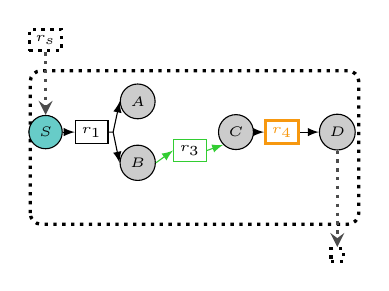
\begin{tikzpicture}[scale=0.39]\tiny
      \tikzstyle{metabolite}=[draw,circle,fill=white!80!black];
      \tikzstyle{repairmetabolite}=[draw,white!40!black, circle,fill=white!90!black,text=white!40!black,dashed];
      \tikzstyle{seed}=[draw,circle,fill=BlueGreen!70];%white!80!black
      \tikzstyle{target}=[draw,circle,fill=YellowOrange];%white!40!black
      \tikzstyle{reaction}=[draw,rectangle];
       \tikzstyle{export}=[draw,rectangle,dotted, very thick];
       \tikzstyle{exportrepair}=[draw,rectangle,dotted, very thick,white!80!black,text=white!70!black];
      \tikzstyle{repairreaction}=[draw,rectangle,white!40!black,text=white!40!black,dashed];
      \tikzstyle{solreaction}=[draw,rectangle,LimeGreen,text=black];
      \tikzstyle{initial}=[->,>=latex,thick];
      \tikzstyle{bdd}=[->,>=latex,thick];
      \tikzstyle{etiq}=[midway,fill=black!20,scale=0.5];
      \tikzstyle{stc}=[draw, rectangle, white, text=black]


      \draw [black,dotted, rounded corners, very thick] (-0.5,4) rectangle (10.2,9);
     % \node (system) [draw, rounded rectangle] at (0,0) {} (7cm,5cm);

      \node[seed] (S) at (0,7) {$S$};
      \node[metabolite] (A) at (3,8) {$A$};
      \node[metabolite] (B) at (3,6) {$B$};
      \node[metabolite] (C) at (6.2,7) {$C$};
      \node[metabolite] (D) at (9.5,7) {$D$};

      \node[reaction] (R1) at (1.5,7) {$r_{1}$};
      \node[reaction, very thick,YellowOrange] (R4) at (7.7,7) {$r_{4}$}; %LimeGreen
      %\node[solreaction] (R2) at (4.7,7.6) {$r_{2}$};
      \node[solreaction] (R3) at (4.7,6.4) {$r_{3}$};

      % R1 : S => A + B
      \draw[->,>=latex] (S.east) -- (R1.west);
      \draw[->,>=latex] (R1.east) -- (2.2,7) -- (A.west);
      \draw[->,>=latex] (2.2,7)  -- (B.west);

      % R2 : A => C
      %\draw[->,>=latex,LimeGreen] (A.east) -- (R2.west);
      %\draw[->,>=latex,LimeGreen] (R2.east) -- (C.north west);

      % R3 : B => C
      \draw[->,>=latex,LimeGreen] (B.east) -- (R3.west);
      \draw[->,>=latex,LimeGreen] (R3.east) -- (C.south west);

      % R4 : C => D
      \draw[->,>=latex] (C.east) -- (R4.west);
      \draw[->,>=latex] (R4.east) -- (D.west);

      %export G
      \node[export] (outD) at (9.5,3) {\ExportReaction};
      \draw[->,>=stealth,white!30!black,dotted, very thick] (D.south) --  (outD.north);

      %import S2
      \node[export] (inS) at (0,10) {$r_{s}$};
      \draw[->,>=stealth,white!30!black,dotted, very thick] (inS) --  (S.north);

  \end{tikzpicture}
% \end{figure}

% \end{document}

      \caption{Topological completion $R_2=\{r_3\}$ satisfies $r_4\in\Activity{t}{G_2}{\{S\}}$ and carries no flux as well, due to accumulation of compound $A$ that contradicts Eq.~\ref{eq:stoichiometric:equation}.\label{gra:union_nf_f2}}
    \end{minipage}
    \begin{minipage}[t]{.32\textwidth}
      \input{union_of_no_flux_has_flux}
      \caption{Completion with the union $R_1\cup R_2=\{r_2,r_3\}$. $G=G_1\cup G_2$  satisfies $r_4\in\Activity{h}{G}{\{S\}}$ and thus is flux-balanced.
      \label{gra:union_nf_f}}
    \end{minipage}
\end{figure}
% ----------------------------------------------------------------------


% ----------------------------------------------------------------------
\begin{figure}
    \captionsetup{width=0.3\textwidth}
    \centering
    \begin{minipage}[t]{.32\textwidth}
      \input{union_of_no_flux_has_no_flux1}
      \caption{Topological completion $R_1=\{r_2\}$ satisfies $r_4\in\Activity{t}{G_1}{\{S\}}$, but carries no flux, due to accumulation of compound $B$ that contradicts Eq.~\ref{eq:stoichiometric:equation}.\label{gra:union_nf_nf1}}
    \end{minipage}
    \begin{minipage}[t]{.32\textwidth}
      \input{union_of_no_flux_has_no_flux2}
      \caption{Topological completion $R_1=\{r_3\}$ satisfies $r_4\in\Activity{t}{G_2}{\{S\}}$, but carries no flux, due to accumulation of compounds $A$ and $E$ that contradicts Eq.~\ref{eq:stoichiometric:equation}.\label{gra:union_nf_nf2}}
    \end{minipage}
    \begin{minipage}[t]{.32\textwidth}
      \input{union_of_no_flux_has_no_flux}
      \caption{Completion with the union $R_1\cup R_2=\{r_2,r_3\}$. $G=G_1\cup G_2$ satisfies $r_4\in\Activity{t}{G}{\{S\}}$, but contradicts minimality and carries no flux $r_4\not \in\Activity{s}{G}{\{S\}}$, due to accumulation of compound $E$ that contradicts Eq.~\ref{eq:stoichiometric:equation}.\label{gra:union_nf_nf}}
    \end{minipage}
\end{figure}
% ----------------------------------------------------------------------



%%% Local Variables:
%%% mode: latex
%%% TeX-master: "paper"
%%% End:


\section{Answer Set Programming with Linear Constraints}\label{sec:background}

For encoding our hybrid problem,
we rely upon the theory reasoning capacities of the ASP system \clingo\ that allows us to extend ASP with linear constraints over reals
(as addressed in Linear Programming).
We confine ourselves below to features relevant to our application and refer the interested reader for details to~\citep{gekakaosscwa16a}.

As usual, a \emph{logic program} consists of \emph{rules} of the form
\begin{lstlisting}[mathescape=true,numbers=none]
   a$_0$ :- a$_1$,...,a$_m$,not a$_{m+1}$,...,not a$_n$
\end{lstlisting}
where each \lstinline[mathescape=true]{a$_i$} is either
a \emph{(regular) atom} of form \lstinline[mathescape=true]{p(t$_1$,...,t$_k$)}
where all \lstinline[mathescape=true]{t$_i$} are terms
or
a \emph{linear constraint atom} of form%
\footnote{In \clingo, theory atoms are preceded by `\texttt{\&}'.}
`\lstinline[mathescape=true]@&sum{w$_1$*x$_1$;$\dots$;w$_l$*x$_l$} <= k@'
that stands for the linear constraint
\(
w_1\cdot x_1+\dots+w_l\cdot x_l\leq k
\).
All \lstinline[mathescape=true]{w$_i$} and \lstinline[mathescape=true]{k} are finite sequences of digits with at most one dot%
\footnote{In the input language of \clingo, such sequences must be quoted to avoid clashes.}
and represent real-valued coefficients $w_i$ and $k$.
Similarly all \lstinline[mathescape=true]{x$_i$} stand for the real-valued variables $x_i$.
%
As usual, \lstinline[mathescape=true]{not} denotes (default) \emph{negation}.
A rule is called a \emph{fact} if $n=0$.

Semantically, a logic program induces a set of \emph{stable models},
being distinguished models of the program determined by stable models semantics~\citep{gellif91a}.
%
Such a stable model $X$ is an \emph{LC-stable model} of a logic program $P$,%
\footnote{This corresponds to the definition of $T$-stable models using a \emph{strict} interpretation of theory atoms~\citep{gekakaosscwa16a},
  and letting $T$ be the theory of linear constraints over reals.}
if there is an assignment of reals to all real-valued variables occurring in $P$ that
(i)     satisfies all linear constraints associated with linear constraint atoms in $P$ being     in $X$
and
(ii) falsifies all linear constraints associated with linear constraint atoms in $P$ being not in $X$.
%
For instance, the (non-ground) logic program containing the fact
`\lstinline[mathescape=true]{a("1.5").}'
along with the rule
`\lstinline[mathescape=true]@&sum{R*x} <= 7 :- a(R).@'
has the stable model
\par
\lstinline[mathescape=true]@$\{$a("1.5")$,\;$&sum{"1.5"*x}<=7$\}$@.
\\
This model is LC-stable since there is an assignment,
e.g.\ $\{x\mapsto 4.2\}$,
that satisfies the associated linear constraint `$1.5*x\leq 7$'.
We regard the stable model along with a satisfying real-valued assignment as a solution to a logic program containing linear constraint atoms.
\review{For a more detailed introduction of ASP extended with linear constraints, illustrated with more complex examples, we refer the interested reader to~\citep{jakaosscscwa17a}.}

To ease the use of ASP in practice,
several extensions have been developed.
First of all, rules with variables are viewed as shorthands for the set of their ground instances.
Further language constructs include
\emph{conditional literals} and \emph{cardinality constraints} \citep{siniso02a}.
The former are of the form
\lstinline[mathescape=true]{a:b$_1$,...,b$_m$},
the latter can be written as
\lstinline[mathescape=true]+s{d$_1$;...;d$_n$}t+,
where \lstinline{a} and \lstinline[mathescape=true]{b$_i$} are possibly default-negated (regular) literals  % for $0\leq i\leq m$,
and each \lstinline[mathescape=true]{d$_j$} is a conditional literal; % for $1\leq i\leq n$;
\lstinline{s} and \lstinline{t} provide optional lower and upper bounds on the number of satisfied literals in the cardinality constraint.
We refer to \lstinline[mathescape=true]{b$_1$,...,b$_m$} as a \emph{condition}.
%
The practical value of both constructs becomes apparent when used with variables.
For instance, a conditional literal like
\lstinline[mathescape=true]{a(X):b(X)}
in a rule's antecedent expands to the conjunction of all instances of \lstinline{a(X)} for which the corresponding instance of \lstinline{b(X)} holds.
%
Similarly,
\lstinline[mathescape=true]+2{a(X):b(X)}4+
is true whenever at least two and at most four instances of \lstinline{a(X)} (subject to \lstinline{b(X)}) are true.
%
Finally, objective functions minimizing the sum of weights $w_i$ subject to condition $c_i$ are expressed as
\lstinline[mathescape=true]!#minimize{$w_1$:$c_1$;$\dots$;$w_n$:$c_n$}!.
% \lstinline[mathescape=true]!#minimize{$w_1$@$l_1$:$c_1$;$\dots$;$w_n$@$l_n$:$c_n$}!.
% Lexicographically ordered objective functions are (optionally) distinguished via levels indicated by $l_i$.

In the same way,
the syntax of linear constraints offers several convenience features.
As above,
elements in linear constraint atoms can be conditioned,
viz.\par
`\lstinline[mathescape=true]@&sum{w$_1$*x$_1$:c$_1$;...;w$_l$*x$_l$:c$_n$} <= k@'
\\
where each \lstinline[mathescape=true]{c$_i$} is a condition.
% Also, linear constraints can be formed with further relations, viz.\
% \texttt{>=},
% \texttt{<},
% \texttt{>},
% \texttt{=},
% and
% \texttt{!=}.
Moreover, the theory language for linear constraints offers a domain declaration for real variables,
`\lstinline[mathescape=true]@&dom{lb..ub} = x@'
expressing that all values of \texttt{x} must lie between \texttt{lb} and \texttt{ub}.
And finally the maximization (or minimization) of an objective function can be expressed with
\lstinline[mathescape=true]@&maximize{w$_1$*x$_1$:c$_1$;...;w$_l$*x$_l$:c$_n$}@
(by \texttt{minimize}).
The full theory grammar for linear constraints over reals is available at~\url{https://potassco.org}.

%%% Local Variables:
%%% mode: latex
%%% TeX-master: "paper"
%%% End:


\section{Heuristic language elements}\label{sec:approach}

We express heuristic modifications via a set $\mathcal{H}$ of \emph{heuristic atoms} 
disjoint from $\mathcal{A}$.
Such a heuristic atom is formed from a dedicated predicate \hpredicate\ along with four arguments:
a (reified) atom $a\in\mathcal{A}$,
a heuristic modifier $m$,
and two  integers $v,p\in\mathbb{Z}$.
A heuristic modifier is used to manipulate the heuristic treatment of an atom $a$ via the 
modifier's value given by $v$.
The role of this value varies for each modifier.
We distinguish four primitive heuristic modifiers:
\begin{description}
\item [\texttt{init}] for initializing the heuristic value of $a$ with $v$,
\item [\texttt{factor}] for amplifying the heuristic value of $a$ by factor $v$,
\item [\texttt{level}] for ranking all atoms; the rank of $a$ is $v$,
\item [\texttt{sign}] for attributing the sign of $v$ as truth value to $a$.
\end{description}
While $v$ allows for changing an atom's heuristic behavior relative to \emph{other} atoms,
the second integer $p$ allows us to express a priority for disambiguating similar
heuristic modifications to the \emph{same} atom.
This is particularly important in our dynamic setting, where varying heuristic atoms may be obtained
in view of the current assignment.
For instance, the heuristic atoms
\hpred{b}{\mathtt{sign}}{1}{3}
and
\hpred{b}{\mathtt{sign}}{-1}{5}
aim at assigning opposite truth values to atom $b$.
This conflict can be resolved by preferring the heuristic modification with the higher priority,
viz.\ 5 in \hpred{b}{\mathtt{sign}}{-1}{5}.
Obviously such priorities can only support disambiguation but not resolve conflicting values sharing the same priority.

For accommodating priorities,
we define for an assignment \ass\ the \emph{preferred values} for modifier $m$ on atom $a$ as
\[
V_{a,m}(\ass)=
\textit{argmax}_{v\in\mathbb{Z}}\{p\mid\Tsigned{\hpred{a}{m}{v}{p}}\in\ass\}.
\]
Heuristic values are dynamic;
they are extracted from the current assignment and may thus vary during solving.
Note that $V_{a,m}(\ass)$ returns the singleton set $\{v\}$,
if the current assignment \ass\ contains a single true heuristic atom \hpred{a}{m}{v}{p} 
involving $a$ and $m$.
$V_{a,m}(\ass)$ is empty whenever there are no such heuristic atoms.
%
And whenever all heuristic atoms regarding $a$ and $m$ have the same priority $p$,
$V_{a,m}(\ass)$ is equivalent to
\(
\{v\mid\Tsigned{\hpred{a}{m}{v}{p}}\in\ass\}
\).

Here are a few examples.
We obtain % the preferred values
$V_{b,\mathtt{sign}}(\ass_1)=\{-1\}$
and
$V_{c,\mathtt{init}}(\ass_1)=\emptyset$
from assignment
\(
\ass_1=\{\Fsigned{a},\Tsigned{\hpred{b}{\mathtt{sign}}{1}{3}},\Tsigned{\hpred{b}{\mathtt{sign}}{-1}{5}}\}
\),
while assignment
\(
\ass_2=\{\Tsigned{\hpred{b}{\mathtt{sign}}{1}{3}},\Tsigned{\hpred{b}{\mathtt{sign}}{-1}{3}}\}
\)
results in $V_{b,\mathtt{sign}}(\ass_2)=\{1,-1\}$.

For ultimately resolving ambiguities among alternative values for heuristic modifiers, 
we propose for a set $V\subseteq\mathbb{Z}$ of integers the function $\nu(V)$ as
\[
%\nu(V)=
\mathit{max}\big(\{v\in V\!\mid v\geq 0\}\cup\{0\}\big)
+
\mathit{min}\big(\{v\in V\!\mid v\leq 0\}\cup\{0\}\big).
\]
Note that $\nu(\emptyset)=0$, attributing 0 the status of a neutral value.
Alternative options exist, like taking means or median of $V$ or even time specific criteria
relating to the emergence of values in the assignment.
%
In the above examples,
we get $\nu(V_{b,\mathtt{sign}}(\ass_1))=-1$ and $\nu(V_{b,\mathtt{sign}}(\ass_2))=0$.

Given this, we proceed by defining the \emph{domain-specific extension} $d$ to the heuristic function $h$ 
for $a\in\mathcal{A}$ as
\[
d_0(a)=\nu(V_{a,\mathtt{init}}(\ass_0))+h_0(a)
\]
and for $i\geq 1$
\[
d_i(a)=
\left\{
  \begin{array}{rl}
    \nu(V_{a,\mathtt{factor}}(\ass_i))\times h_i(a)&\text{if } V_{a,\mathtt{factor}}(\ass_i)\neq\emptyset
    \\
                                             h_i(a)&\text{otherwise}
  \end{array}
\right.
\]
First of all, it is important to note that $d$ is merely a modification and not a replacement of the
system heuristic $h$.
In fact, $d$ extends the range of $h$ to $(-\infty,+\infty)$.
Negative values serve as penalties.
The values of the \texttt{init} modifiers are added to $h_0$ in $d_0$.
The use of addition rather than multiplication allows us to override an initial value of 0.
Also, the higher the absolute value of the \texttt{init} modifier, the longer lasts its effect
(given the decay of heuristic values).
Unlike this, \texttt{factor} modifiers rely on multiplication because they aim at de- or increasing
conflict scores gathered during conflict analysis.
In view of $h$'s range,
a factor greater than 1 amplifies the score, a negative one penalizes the atom, and 0 resets the atom's score.
Enforcing a factor of 1 
% (for instance, through assigning a high priority)
transfers control back to the system heuristic $h$.

Heuristically modified logic programs are simply programs over $\mathcal{A}\cup\mathcal{H}$,
the original vocabulary extended by heuristic atoms (without restrictions).
As a first example,
let us extend our planning encoding by a rule favoring atoms expressing action occurrences close to
the goal situation.
\begin{lstlisting}
_h(occ(A,T),factor,T,0) :- action(A),time(T).
\end{lstlisting}
With \texttt{factor}, we impose a bias on the underlying heuristic function $h$.
Rather than comparing, for instance,
the plain values $h(\mathtt{occ(a,2)})$ and $h(\mathtt{occ(a,3)})$,
a decision is made by looking at $2\times h(\mathtt{occ(a,2)})$ and  $3\times h(\mathtt{occ(a,3)})$,
even though it still depends on $h$.
A further refined strategy may suggest considering climbing actions as early as possible.
\begin{lstlisting}
_h(occ(climb,T),factor,l-T,1) :- time(T).
\end{lstlisting}
Clearly, this rule conflicts with the more general rule above.
However, this conflict is resolved in favor of the more specific rule by attributing it a higher
priority (viz.~1 versus 0).

% Similar statements can be formulated with the \texttt{init} modifier in order to change the initial heuristic values.

For capturing a \emph{domain-specific extension} $t$ to the sign heuristic $s$,
we define for $a\in\mathcal{A}$ and $i\geq 0$:
\[
t_i(a)=
\left\{
  \begin{array}{rl}
    \true &\text{if }
           \nu(V_{a,\mathtt{sign}}(\ass_i))>0
           % \text{ and }
           % V_{a,\mathtt{sign}}(\ass_i)\neq\emptyset
           \\
    \false&\text{if }
           \nu(V_{a,\mathtt{sign}}(\ass_i))<0
           % \text{ and }
           % V_{a,\mathtt{sign}}(\ass_i)\neq\emptyset
           \\
    s_i(a)&\text{otherwise}
  \end{array}
\right.
\]
As with $d$ above, the extension $t$ to the sign heuristic is dynamic.
The sign of the modifier's preferred value determines the truth value to assign to an atom at hand.
No \texttt{sign} modifier (or enforcing a value of 0) leaves sign selection with the system's sign heuristic $s$.
%
For example, the heuristic rule
\begin{lstlisting}
_h(holds(F,T),sign,-1,0) :- fluent(F),time(T).
\end{lstlisting}
tells the solver to assign false to non-deterministically chosen fluents.
%
The next pair of rules is a further refinement of our strategy on climbing actions,
favoring their effective occurrence in the first half of the plan.
\begin{lstlisting}
_h(occ(climb,T),sign, 1,0) :- T<l/2,time(T).
_h(occ(climb,T),sign,-1,0) :- T>l/2,time(T).
\end{lstlisting}
Thus, while the atom $\mathtt{occ(climb,1)}$ is preferably made true,
false should rather be assigned to $\mathtt{occ(climb,l)}$.

Finally, for accommodating rankings induced by \texttt{level} modifiers,
we define for an assignment \ass\ and $\mathcal{A}'\subseteq\mathcal{A}$:
\[
\ell_\ass(\mathcal{A}')=\textit{argmax}_{a\in\mathcal{A}'}\nu(V_{a,\mathtt{level}}(\ass))
\]
The set $\ell_\ass(\mathcal{A}')$ gives all atoms in $\mathcal{A}'$ with the highest \texttt{level} values relative to
the current assignment \ass.
Similar to $d$ and $t$ above, this construction is also dynamic and the rank of atoms may vary during solving.
The function $\ell_\ass$ is then used to modify the selection of unassigned atoms in the above elaboration of \textit{decide}.
For this purpose, we replace Item~2 by
\(
U:=\ell_\ass(\mathcal{A}\setminus (\tlits{\ass}\cup\flits{\ass}))
\)
in order to restrict $U$ to unassigned atoms of (current) highest rank.
Unassigned atoms at lower levels are only considered once all atoms at higher levels have been assigned.
Atoms without an associated level default to level 0 because $\nu(\emptyset)=0$.
Hence, negative levels act as a penalty since the respective atoms are only taken into account
once all atoms with non-negative or no associated level have been assigned.

For a complementary example, 
consider a \texttt{level}-based formulation of the previous (\texttt{factor}-based) heuristic rule.
\begin{lstlisting}
_h(occ(A,T),level,T,0) :- action(A),time(T).
\end{lstlisting}
Unlike the above, $\mathtt{occ(a,2)}$ and $\mathtt{occ(a,3)}$ are now associated with different ranks,
which leads to strictly preferring $\mathtt{occ(a,3)}$ over $\mathtt{occ(a,2)}$ 
whenever both atoms are unassigned.
Hence, \texttt{level} modifiers partition the set of atoms and restrict $h$ to unassigned atoms at the highest level.

The previous replacement along with the above amendments of $h$ and $s$ through the domain-specific extensions $d$ and $t$
yields the following elaboration of CDCL's heuristic choice operation \textit{decide} for $i\geq 1$ (and given $d_0$).$^{\ref{fn:ass}}$
% --------------------------------------------------
\begin{enumerate}\addtocounter{enumi}{-1}\itemindent 10pt
\item $h_{i-1}(a) := d_{i-1}(a)$                         \hfill for each $a\in\mathcal{A}\qquad$
\item $h_i(a) := \alpha_i\times h_{i-1}(a) + \beta_i(a)$ \hfill for each $a\in\mathcal{A}\qquad$
\item $U:=\ell_{\ass_{i-1}}(\mathcal{A}\setminus (\tlits{\ass_{i-1}}\cup\flits{\ass_{i-1}}))$
\item $C:= \textit{argmax}_{a\in U}d_i(a)$
\item $a:= \tau(C)$
\item $\ass_i := \ass_{i-1}\cup\{t_i(a)a\}$
\end{enumerate}
% --------------------------------------------------
Although we formally model both $h$ and $d$ (as well as $s$ and $t$) as functions,
there is a substantial conceptual difference in practice in that $h$ is a system-specific data structure while $d$ is an associated method.
This is also reflected above, where $h$ is subject to assignments.
%
Item~0 makes sure that our heuristic modifications take part in the look-back based evolution in Item~1,
and are thus also subject to decay.
We added this as a separate line rather than integrating it into Item~1 in order to stress that our
modifications are modular in leaving the underlying heuristic machinery unaffected.
%
Item~2 gathers in $U$ all unassigned atoms of highest rank.
%
Among them, Item~3 collects in $C$ all atoms $a$ with a maximum heuristic value $d_i(a)$.
%
Since this is not guaranteed to yield a unique element, the system-specific tie-breaking function
$\tau$ is evoked to return a unique atom.
%
Finally, the modified sign heuristic $t_i$ determines a truth value for $a$, and the resulting
signed literal ${t_i(a)a}$ is added to the current assignment.

Note that so far all sample heuristic rules were \emph{static} in the sense that they are turned into
facts by the grounder and thus remain unchanged during solving.
Examples of dynamic heuristic rules are given at the end of next section.

Our simple heuristic language is easily extended by further heuristic atoms.
For instance, \hpred{a}{\mathtt{true}}{v}{p} and \hpred{a}{\mathtt{false}}{v}{p} have turned out to be useful in practice.
\begin{lstlisting}
_h(A,level,V,P) :- _h(A,true, V,P).
_h(A,sign, 1,P) :- _h(A,true, V,P).
_h(A,level,V,P) :- _h(A,false,V,P).
_h(A,sign,-1,P) :- _h(A,false,V,P).
\end{lstlisting}
%
For instance, the heuristic atom \hpred{a}{\mathtt{true}}{3}{3} expands to 
\hpred{a}{\mathtt{level}}{3}{3} and \hpred{a}{\mathtt{sign}}{1}{3},
expressing a preference for both making a decision on~$a$ and
assigning it to true.
On the other hand,
\hpred{a}{\mathtt{false}}{-3}{3} expands to 
\hpred{a}{\mathtt{level}}{-3}{3} and \hpred{a}{\mathtt{sign}}{-1}{3},
thus suggesting not to make a decision on~$a$ but to
assign it to false if there is no ``better'' decision variable.

Another shortcut of pragmatic value is the abstraction from specific priorities.
For this, we use the following rule.
\begin{lstlisting}
_h(A,M,V,#abs(V)) :- _h(A,M,V).
\end{lstlisting}
With it,
we can directly describe the heuristic restriction used in \cite{rintanen11a} to simulate planning
by iterated deepening $A^*$ \cite{korf85a} in SAT solving through limiting choices to action variables,
assigning those for time \texttt{T} before those for time \texttt{T+1}, and always assigning truth
value \texttt{true} (where \texttt{l} is a constant indicating the planning horizon):
\begin{lstlisting}
_h(occ(A,T),true,l-T) :- action(A), time(T).
\end{lstlisting}

Although we impose no restriction on the occurrence of heuristic atoms within logic programs,
it seems reasonable to require that the addition of rules containing heuristic atoms does not alter
the stable models of the original program.
That is, given a logic program $P$ over $\mathcal{A}$ and a set of rules $H$ over $\mathcal{A}\cup\mathcal{H}$,
we aim at a one-to-one correspondence between the stable models of $P$ and $P\cup H$ and
their identity upon projection on $\mathcal{A}$.
This property is guaranteed whenever heuristic atoms occur only in the head of rules and thus only
depend upon regular atoms.
In fact, so far, this class of rules turned out to be expressive enough to model all heuristics of interest,
including the ones presented in this paper.
It remains future work to see whether more sophisticated schemes, eg., involving recursion, are useful.

%%% Local Variables: 
%%% mode: latex
%%% TeX-master: "paper"
%%% End: 

\section{Experiments}\label{sec:experiments}
%
\begin{table}[t]
\caption{Comparison of approximation techniques by 
(a) runtime and timeouts,
(b) diversification quality, and
(c) minimum distance}
\small
\parbox{.32\linewidth}{\centering
\begin{tabular}{|l||r|r|}

\hline
Class & \textit{T} & \textit{TO}  \\ 
\hline
\Alabel{3} & \textbf{165} & \textbf{70} \\
\Alabel{3}-\textit{true} & 200 & 113 \\ 
\Alabel{3}-\textit{all} & 202 & 118 \\ 
\Alabel{3}-\textit{rd} & 277 & 280 \\ 
\Alabel{3}-\textit{pg} & 317 & 351\\
\Alabel{3}-\textit{pg-l-rd} & 354 & 442\\
\Alabel{3}-\textit{false} & 351 & 443 \\ 
\Alabel{3}-\textit{pg-l} & 351 & 443\\
\Alabel{2}-\textit{true} & 482 & 618\\
\Alabel{2}-\textit{rd} & 474 & 648\\
\Alabel{1} & 482 & 672\\
\Alabel{2}-\textit{dist-to} & 528 & 689\\
\Alabel{2}-\textit{all} & 515 & 696\\
\Alabel{2}-\textit{false} & 532 & 696\\
\Alabel{2}-\textit{pg} & 542 & 708\\
\Alabel{2}-\textit{dist} & 572 & 773\\
\hline
\end{tabular} 
}
\parbox{.32\linewidth}{\centering
\begin{tabular}{|l||r|r|}

\hline
Class & \textit{S} & \textit{avg}\\ 
\hline
\Alabel{1} & \textbf{15} & 0.13\\
\Alabel{2}-\textit{dist-to} & 14 & 0.14\\ 
\Alabel{2}-\textit{pg} & 13 & \textbf{0.18}\\ 
\Alabel{3}-\textit{pg-l} & 11 & 0.17\\
\Alabel{3}-\textit{pg-l-rd} & 10 & 0.16\\
\Alabel{2}-\textit{all}  & 10 & 0.15\\
\Alabel{2}-\textit{dist} & 8 & 0.07\\ 
\Alabel{2}-\textit{false} & 8 & 0.15\\ 
\Alabel{2}-\textit{true} & 7 & 0.12\\ 
\Alabel{3}-\textit{false} & 6 & 0.16\\ 
\Alabel{2}-\textit{rd} & 5 & 0.12\\ 
\Alabel{3}-\textit{all}  & 5 & 0.08 \\ 
\Alabel{3}-\textit{true} & 4 & 0.08 \\ 
\Alabel{3}-\textit{rd} & 2 & 0.09 \\ 
\Alabel{3}-\textit{pg} & 1 & 0.09\\
%\Alabel{3}-Hdyn & 1 & 0.09\\ 
\Alabel{3} & 0 & 0.06\\

\hline
\end{tabular} 
}
\parbox{.32\linewidth}{\centering
\begin{tabular}{|l||r|r|}

\hline
Class & \textit{S} & \textit{avg}\\ 
\hline
\Alabel{1} & \textbf{15} & 12.25\\
\Alabel{2}-\textit{dist-to} & 13 & 10.38\\
\Alabel{3}-\textit{pg-l-rd } & 13 & 11.82 \\
\Alabel{2}-\textit{dist} & 12 & 5.31\\
\Alabel{3}-\textit{pg-l} & 12 & 11.10\\
\Alabel{2}-\textit{pg} & 10 & \textbf{12.86}\\
\Alabel{2}-\textit{rd} & 9 & 8.77 \\
\Alabel{3}-\textit{all}  & 7 & 3.99 \\ 
\Alabel{3}-\textit{true} & 6 & 4.00 \\ 
\Alabel{3}-\textit{false} & 6 & 7.07 \\ 
\Alabel{2}-\textit{false} & 6 & 6.80\\
\Alabel{2}-\textit{all}  & 4 & 6.98\\
\Alabel{2}-\textit{true} & 3 & 5.31\\
\Alabel{3}-\textit{rd} & 2 & 6.43\\
\Alabel{3} & 2 & 4.28\\
%\Alabel{3}-Hdyn & 1 & 2.90\\ 
\Alabel{3}-\textit{pg} & 0 & 2.79\\
\hline
\end{tabular} 
}
\label{tab:time_comparison_small}
\label{tab:diverse_comparison_small}
\label{tab:min_dist_comparison_small}
\end{table}
%
In this section, we present experiments focusing on the \emph{approximation} techniques of the \asprin\ system for obtaining most dissimilar optimal
solutions. 
%
While \emph{enumeration} and \emph{replication} provide exact results, they need to calculate and store a possibly exponential number of optimal
models or deal with a large search space, respectively.
%
Those techniques are therefore not effective for most practical applications.
%
For Algorithm~\Alabel{2}, we considered the variations \textit{rd}, \textit{pg}, \textit{true}, \textit{false}, and \textit{all} .
%
In \textit{dist}, we issued no timeout for the computation of the partial interpretation, 
while in \textit{dist-to}, we set a timeout for this computation of half the total possible runtime.
%
For Algorithm~\Alabel{3}, we consider the variations that include no extra ASP computation, namely, 
\textit{rd}, \textit{pg}, \textit{true}, \textit{false}, and \textit{all} .
%
We also evaluated a version without any heuristic modification (named simply \Alabel{3}).
%
Furthermore, following \cite{nadel11a}, 
we considered a variation of \textit{pg}, viz.~\textit{pg-l}, 
where the atoms of the selected partial interpretation are given a higher priority, 
and \textit{pg-l-rd}, extending \textit{pg-l} by fixing initially a random sign to all atoms not appearing in the partial interpretation.

We gathered 186 instances from six different classes: \emph{Design Space exploration (DSE)} from~\cite{angeglharesc13a}, \emph{Timetabling (CTT)}
from~\cite{basotainsc13a}, \emph{Crossing minimization} from the ASP competition 2013, \emph{Metabolic network expansion} from \cite{schthi09a},
\emph{Biological network repair} from \cite{geguivscsithve10a} and \emph{Circuit Diagnosis} from~\cite{sidiqqi11a}.
Since we required instances with multiple optimal solutions, we exclusively focused on Pareto optimality. 
DSE and CTT are inherently multi-objective and therefore we could naturally define a Pareto preference for them. 
For the other classes, we turned single-objective into multi-objective optimization problems by distributing their optimization statements.
First, we split the atoms in the optimization statements into four or eight groups evenly. 
We chose for each group the same preference type, either cardinality or subset minimization, and aggregated them by means of Pareto preference.
We calculated optimal solutions regarding these Pareto preferences.
The same was done for CTT and DSE.
An instance was selected if for some Pareto preference ten optimal solutions could be obtained within 600 seconds by \asprin. 
This method generated 816 instances in total. 
We ran the benchmarks on a cluster of Linux machines with dual Xeon E5520 quad-core 2.26 GHz processors and 48 GB RAM. 
We restricted the runtime to 600 seconds and the memory usage to 20 GB RAM.

Since algorithms~\Alabel{1} and \Alabel{2} involve querying programs over preferences, 
we started by evaluating the different query techniques. 
%
For that, we executed \Alabel{1} with query methods \Qlabel{1} to \Qlabel{4} on all selected instances,
stopping after the first $\mathit{solveQuery}$ call was finished.
%
%We achieved that by first calculating an optimal solution and then finding another optimal solution fulfilling the query that the model has to be dissimilar.
The performance of query techniques \Qlabel{2}, \Qlabel{3}, and \Qlabel{4} was similar regarding runtime and only \Qlabel{1} was clearly worse.
We selected \Qlabel{4} for the remaining experiments due to its slightly lower runtime. 
For more detailed tables, we refer to~\cite{roscwa16b}. % \ref{sec:suptables}.

Next, we approximated four most diverse optimal models with methods \Alabel{1} to \Alabel{3}. 
%
We measured runtime and two quality measures.
The first, called diversification quality~\cite{nadel11a},
gives the sum of the Hamming distances among all pairs of solutions normalized to values between zero and one.
The second is the minimum distance among all pairs of solutions of a set in percent.
%
The solution set size of four was chosen because~\cite{shimazu01a} 
claims that three solutions is the optimal amount for a user,
and considering one additional solution provides further insight into the different quality measures. 
%
For all algorithms that do not use heuristics for diversification, 
we instead enabled heuristics preferring a negative sign for the atoms appearing in preference statements. 
This was observed in~\cite{brderosc15b} to improve performance.

Table~\ref{tab:time_comparison_small}(a) provides in column \textit{T} the average runtime and in column \textit{TO} the sum of timeouts. 
The different methods are ordered by the number of timeouts. 
The best results in a column are shown in bold. 
We see that \Alabel{3} is by far the fastest with 70 timeouts, solving 91\% of the instances. 
Heuristic variations of \Alabel{3} perform the best after that. 
Less invasive heuristics achieve similar runtimes with 113-118 timeouts.
More sophisticated heuristics perform worse at 349-443 timeouts.
In a range from 618 to 773 timeouts, non-heuristic methods solve the least instances by a significant margin.
The results are in tune with the nature of the methods. 
Heuristics modifying the solving process for diversity decrease the performance 
in comparison with solving heuristics aimed at performance, 
but not as much as more complex methods involving preferences over optimal models. 

In particular, non-heuristic methods show many timeouts. 
If we tried to analyze the quality of the solutions by assuming worst possible values for the instances that timed out,
the results would be dominated by these instances. 
To avoid that, we calculated a score independent of the runtime.
We considered all possible parings of the different methods. 
For each pair, we compared only instances where both found a solution set.
The method with better quality value for the majority of instances receives a point. 
Finally, we ordered the subsequent tables according to that score. 
 
In Table~\ref{tab:diverse_comparison_small}(b), for each method we see the score in column \textit{S}, and 
the average of the diversification quality (over the instances solved by the method) in column \textit{avg}. 
This way, we can examine the quality a method has achieved compared to other methods, and also the individual average quality.
\Alabel{1} has the best quality with a score of 15, followed by \Alabel{2}-\textit{dist-to}, \Alabel{2}-\textit{pg}, \Alabel{3}-\textit{pg-l} and \Alabel{3}-\textit{pg-l-rd}.
All of those techniques regard the whole previous solution set to calculate the next solution
and guide the solving strictly to diversity.
\Alabel{2}-\textit{pg}, \Alabel{3}-\textit{pg-l} and \Alabel{3}-\textit{pg-l-rd } are also the first, second and third place, respectively, for average diversification quality. 
Next, with scores ranging from 10-7, we see \Alabel{2} methods 
that do not take into account the whole previous set, 
or that were simply unable to find many solutions at all, as in the case of \Alabel{2}-\textit{dist}. 
Finally, we observe that \Alabel{3} variations only regarding the last solution or no previous information 
perform worst in score and average. 
In these cases, the heuristic does not seem to be strong enough to steer the solving to high quality solution sets, 
and \Alabel{3} uses no heuristic or optimization techniques to ensure diverse solutions.

In analogy to Table~\ref{tab:diverse_comparison_small}(b),
Table~\ref{tab:min_dist_comparison_small}(c) provides information for the minimum distance among the solutions. 
%
% The overall grouping of the methods is similar to Table~\ref{tab:diverse_comparison_small}(b). 
%
The best methods considering score and average minimum distance, 
viz.\ \Alabel{1}, \Alabel{2}-\textit{dist-to}, \Alabel{3}-\textit{pg-l-rd}, \Alabel{3}-\textit{pg-l}, \Alabel{2}-\textit{pg}, utilize information from the whole
previous solution set and have strict diversification techniques. 
%\comment{I cut the part about the different behavior of min distance and diversification. The data is not that clear and it saves space. Maybe if we have space left in the end...}

Overall, plain heuristic methods perform better in regards to runtime 
while more complex methods, depending on all previous solutions, lead to better quality. 
%
Furthermore, \Alabel{3}-\textit{pg-l-rd } and \Alabel{3}-\textit{pg-l} provide the best trade-off between performance and quality. 
%
While \Alabel{1}, \Alabel{2}-\textit{dist-to} and \Alabel{2}-\textit{pg} achieve higher quality, they could solve only 18\%, 16\% and 13\% of the instances. 
%
On the other hand, \Alabel{3}-\textit{pg-l-rd } and \Alabel{3}-\textit{pg-l} provide good diversification quality and minimum distance while solving 46\% of the instances. 
%
%\comment{this section is enough for general conclusion: plain heuristic: fast but bad, maxmin: slow but good, more complex heuristic: tradeoff}


%%% Local Variables: 
%%% mode: latex
%%% TeX-master: "paper"
%%% End: 


\section{Discussion}\label{sec:discussion}

We presented a comprehensive framework for computing diverse (or similar) solutions to logic programs with generic preferences
and implemented it in \asprin~2, available at~\cite{asprin}. %\comment{T: Make it available!}
To this end, we introduced a spectrum of different methods, among them, generalizations of existing work to the case of
programs with general preferences.
Hence, certain fragments of our framework provide implementations of the proposals in \cite{eiererfi13a,zhutru13a}.
While the latter had to resort to solver wrappers or even internal solver modifications,
\asprin\ heavily relies upon multi-shot solving that allows for an easy yet fine-grained control of reasoning processes.
Moreover, we provided several generic building blocks, such as 
\textit{maxmin} (and \textit{minmax}) preferences,
query-answering for programs with preferences,
preferences among optimal models,
and an automated approach for the guess and check methodology of~\cite{eitpol06a},
all of which are also of interest beyond diversification.
%
Finally, we took advantage of the uniform setting offered by \asprin~2 to conduct a 
comparative empirical analysis of the various methods for diversification.
Generally speaking,
there is a clear trade-off between performance and diversification quality, 
which allows for selecting the most appropriate method 
depending on the hardness of the application at hand.
%\comment{T: Last phrase is a bit weak\dots}
% \begin{itemize}
% \item System for diverse optimal models of logic program with preferences.
% \item Lifts previous approaches in ASP \cite{eiererfi13a} or with answer set optimization \cite{zhutru13a} to general preferences of \asprin.
% \item Variety of methods.
% \item Experimental evaluation shows that different methods differ wrt performance and diversity of solutions.
% \item There is a tradeoff between performance and diversity, which allows for selecting the most appropiate method at hand for the application at hand.
% \item Furthermore, four more general contributions to preferences: $maxmin$, automation of generate and test, query solving, and preferences over
% optimal models.
% \item Future work: Real world applications on DSS and TT.
% \item Future work: Apply SMT framework of \clingo\ 5. In \cite{eiererfi13a}, the modification of the solver was more efficient than ASP implementation.
%       We intend to do it in a principled (general?) way inside the new framework.
% \end{itemize}



%%% Local Variables: 
%%% mode: latex
%%% TeX-master: "paper"
%%% End: 

\paragraph{Acknowledgments}

This work was partially funded by DFG grants SCHA~550/9 and~11,
as well as the Academy of Finland grant 251170.

%%% Local Variables: 
%%% mode: latex
%%% TeX-master: "paper"
%%% End: 

\bibliographystyle{acmtrans}
\bibliography{lit,procs,akku,bibioinfo} % https://svn.cs.uni-potsdam.de/svn/reposWV/Papers/bibfiles/trunk
%\begin{thebibliography}{}

\bibitem[\protect\citeauthoryear{Banbara, Gebser, Inoue, Ostrowski, Peano,
  Schaub, Soh, Tamura, and Weise}{Banbara
  et~al\mbox{.}}{2015}]{bageinospescsotawe15a}
{\sc Banbara, M.}, {\sc Gebser, M.}, {\sc Inoue, K.}, {\sc Ostrowski, M.}, {\sc
  Peano, A.}, {\sc Schaub, T.}, {\sc Soh, T.}, {\sc Tamura, N.}, {\sc and} {\sc
  Weise, M.} 2015.
\newblock aspartame: Solving constraint satisfaction problems with answer set
  programming.
\newblock In {\em Proceedings of the Thirteenth International Conference on
  Logic Programming and Nonmonotonic Reasoning (LPNMR'15)}, {F.~Calimeri},
  {G.~Ianni}, {and} {M.~Truszczy{\'n}ski}, Eds. Lecture Notes in Artificial
  Intelligence, vol. 9345. Springer-Verlag, 112--126.

\bibitem[\protect\citeauthoryear{Banbara, Kaufmann, Ostrowski, and
  Schaub}{Banbara et~al\mbox{.}}{2017}]{bakaossc16a}
{\sc Banbara, M.}, {\sc Kaufmann, B.}, {\sc Ostrowski, M.}, {\sc and} {\sc
  Schaub, T.} 2017.
\newblock Clingcon: The next generation.
\newblock {\em Theory and Practice of Logic Programming\/}.
\newblock To appear.

\bibitem[\protect\citeauthoryear{Baral}{Baral}{2003}]{baral02a}
{\sc Baral, C.} 2003.
\newblock {\em Knowledge Representation, Reasoning and Declarative Problem
  Solving}.
\newblock Cambridge University Press.

\bibitem[\protect\citeauthoryear{Barrett, Sebastiani, Seshia, and
  Tinelli}{Barrett et~al\mbox{.}}{2009}]{baseseti09a}
{\sc Barrett, C.}, {\sc Sebastiani, R.}, {\sc Seshia, S.}, {\sc and} {\sc
  Tinelli, C.} 2009.
\newblock Satisfiability modulo theories.
\newblock In {\em Handbook of Satisfiability}, {A.~Biere}, {M.~Heule}, {H.~{van
  Maaren}}, {and} {T.~Walsh}, Eds. Frontiers in Artificial Intelligence and
  Applications, vol. 185. IOS Press, Chapter~26, 825--885.

\bibitem[\protect\citeauthoryear{Bartholomew and Lee}{Bartholomew and
  Lee}{2014}]{barlee14b}
{\sc Bartholomew, M.} {\sc and} {\sc Lee, J.} 2014.
\newblock System aspmt2smt: Computing {ASPMT} theories by {SMT} solvers.
\newblock In {\em Proceedings of the Fourteenth European Conference on Logics
  in Artificial Intelligence (JELIA'14)}, {E.~Ferm\'{e}} {and} {J.~Leite}, Eds.
  Lecture Notes in Artificial Intelligence, vol. 8761. Springer-Verlag,
  529--542.

\bibitem[\protect\citeauthoryear{Cabalar, Otero, and Pose}{Cabalar
  et~al\mbox{.}}{2000}]{caotpo00a}
{\sc Cabalar, P.}, {\sc Otero, R.}, {\sc and} {\sc Pose, S.} 2000.
\newblock Temporal constraint networks in action.
\newblock In {\em Proceedings of the Fourteenth European Conference on
  Artificial Intelligence (ECAI'00)}, {W.~Horn}, Ed. IOS Press, 543--547.

\bibitem[\protect\citeauthoryear{Carro and King}{Carro and
  King}{2016}]{iclp-lipics16}
{\sc Carro, M.} {\sc and} {\sc King, A.}, Eds. 2016.
\newblock {\em Technical Communications of the Thirty-second International
  Conference on Logic Programming (ICLP'16)}. Vol.~52. Open Access Series in
  Informatics (OASIcs).

\bibitem[\protect\citeauthoryear{Cotton and Maler}{Cotton and
  Maler}{2006}]{cotmal06a}
{\sc Cotton, S.} {\sc and} {\sc Maler, O.} 2006.
\newblock Fast and flexible difference constraint propagation for {DPLL (T)}.
\newblock In {\em Proceedings of the Ninth International Conference on Theory
  and Applications of Satisfiability Testing (SAT'06)}, {A.~Biere} {and}
  {C.~Gomes}, Eds. Lecture Notes in Computer Science, vol. 4121.
  Springer-Verlag, 170--183.

\bibitem[\protect\citeauthoryear{Crawford and Baker}{Crawford and
  Baker}{1994}]{crabak94a}
{\sc Crawford, J.} {\sc and} {\sc Baker, A.} 1994.
\newblock Experimental results on the application of satisfiability algorithms
  to scheduling problems.
\newblock In {\em Proceedings of the Twelfth National Conference on Artificial
  Intelligence (AAAI'94)}, {B.~Hayes-Roth} {and} {R.~Korf}, Eds. AAAI Press,
  1092--1097.

\bibitem[\protect\citeauthoryear{Dantzig}{Dantzig}{1963}]{dantzig63a}
{\sc Dantzig, G.} 1963.
\newblock {\em Linear Programming and Extensions}.
\newblock Princeton University Press.

\bibitem[\protect\citeauthoryear{{De Rosis}, Eiter, Redl, and Ricca}{{De Rosis}
  et~al\mbox{.}}{}]{roeireri15a}
{\sc {De Rosis}, A.}, {\sc Eiter, T.}, {\sc Redl, C.}, {\sc and} {\sc Ricca,
  F.}
\newblock Constraint answer set programming based on {HEX}-programs.

\bibitem[\protect\citeauthoryear{Drescher and Walsh}{Drescher and
  Walsh}{2010}]{drewal10a}
{\sc Drescher, C.} {\sc and} {\sc Walsh, T.} 2010.
\newblock A translational approach to constraint answer set solving.
\newblock {\em Theory and Practice of Logic Programming\/}~{\em 10,\/}~4-6,
  465--480.

\bibitem[\protect\citeauthoryear{Gebser, Kaminski, Kaufmann, Ostrowski, Schaub,
  and Wanko}{Gebser et~al\mbox{.}}{2016}]{gekakaosscwa16a}
{\sc Gebser, M.}, {\sc Kaminski, R.}, {\sc Kaufmann, B.}, {\sc Ostrowski, M.},
  {\sc Schaub, T.}, {\sc and} {\sc Wanko, P.} 2016.
\newblock Theory solving made easy with clingo~5.
\newblock See \citeN{iclp-lipics16}, 2:1--2:15.

\bibitem[\protect\citeauthoryear{Gebser, Kaminski, Kaufmann, and Schaub}{Gebser
  et~al\mbox{.}}{2014}]{gekakasc14b}
{\sc Gebser, M.}, {\sc Kaminski, R.}, {\sc Kaufmann, B.}, {\sc and} {\sc
  Schaub, T.} 2014.
\newblock \textit{Clingo} = {ASP} + control: Preliminary report.
\newblock In {\em Technical Communications of the Thirtieth International
  Conference on Logic Programming (ICLP'14)}, {M.~Leuschel} {and}
  {T.~Schrijvers}, Eds. Theory and Practice of Logic Programming, Online
  Supplement, vol. arXiv:1405.3694v1.
\newblock Available at \url{http://arxiv.org/abs/1405.3694v1}.

\bibitem[\protect\citeauthoryear{Gebser, Kaufmann, and Schaub}{Gebser
  et~al\mbox{.}}{2012}]{gekasc09c}
{\sc Gebser, M.}, {\sc Kaufmann, B.}, {\sc and} {\sc Schaub, T.} 2012.
\newblock Conflict-driven answer set solving: From theory to practice.
\newblock {\em Artificial Intelligence\/}~{\em 187-188}, 52--89.

\bibitem[\protect\citeauthoryear{Gelfond and Lifschitz}{Gelfond and
  Lifschitz}{1991}]{gellif91a}
{\sc Gelfond, M.} {\sc and} {\sc Lifschitz, V.} 1991.
\newblock Classical negation in logic programs and disjunctive databases.
\newblock {\em New Generation Computing\/}~{\em 9}, 365--385.

\bibitem[\protect\citeauthoryear{Goldberg}{Goldberg}{1991}]{goldberg91a}
{\sc Goldberg, D.} 1991.
\newblock What every computer scientist should know about floating-point
  arithmetic.
\newblock {\em ACM Computing Surveys (CSUR)\/}~{\em 23,\/}~1, 5--48.

\bibitem[\protect\citeauthoryear{Janhunen, Liu, and Niemelä}{Janhunen
  et~al\mbox{.}}{2011}]{jalini11a}
{\sc Janhunen, T.}, {\sc Liu, G.}, {\sc and} {\sc Niemelä, I.} 2011.
\newblock Tight integration of non-ground answer set programming and
  satisfiability modulo theories.
\newblock In {\em Proceedings of the First Workshop on Grounding and
  Transformation for Theories with Variables (GTTV'11)}, {P.~Cabalar},
  {D.~Mitchell}, {D.~Pearce}, {and} {E.~Ternovska}, Eds. 1--13.

\bibitem[\protect\citeauthoryear{Lierler and Susman}{Lierler and
  Susman}{2016}]{liesus16a}
{\sc Lierler, Y.} {\sc and} {\sc Susman, B.} 2016.
\newblock {SMT}-based constraint answer set solver {EZSMT} (system
  description).
\newblock See \citeN{iclp-lipics16}, 1:1--1:15.

\bibitem[\protect\citeauthoryear{Liu, Janhunen, and Niemelä}{Liu
  et~al\mbox{.}}{2012}]{lijani12a}
{\sc Liu, G.}, {\sc Janhunen, T.}, {\sc and} {\sc Niemelä, I.} 2012.
\newblock Answer set programming via mixed integer programming.
\newblock In {\em Proceedings of the Thirteenth International Conference on
  Principles of Knowledge Representation and Reasoning (KR'12)}, {G.~Brewka},
  {T.~Eiter}, {and} {S.~McIlraith}, Eds. AAAI Press, 32--42.

\bibitem[\protect\citeauthoryear{Simons, Niemelä, and Soininen}{Simons
  et~al\mbox{.}}{2002}]{siniso02a}
{\sc Simons, P.}, {\sc Niemelä, I.}, {\sc and} {\sc Soininen, T.} 2002.
\newblock Extending and implementing the stable model semantics.
\newblock {\em Artificial Intelligence\/}~{\em 138,\/}~1-2, 181--234.

\bibitem[\protect\citeauthoryear{Soh, Inoue, Tamura, Banbara, and
  Nabeshima}{Soh et~al\mbox{.}}{2010}]{sointabana10a}
{\sc Soh, T.}, {\sc Inoue, K.}, {\sc Tamura, N.}, {\sc Banbara, M.}, {\sc and}
  {\sc Nabeshima, H.} 2010.
\newblock A {SAT}-based method for solving the two-dimensional strip packing
  problem.
\newblock {\em Fundamenta Informaticae\/}~{\em 102,\/}~3-4, 467--487.

\bibitem[\protect\citeauthoryear{Taillard}{Taillard}{1993}]{taillard93a}
{\sc Taillard, E.} 1993.
\newblock Benchmarks for basic scheduling problems.
\newblock {\em European Journal of Operational Research\/}~{\em 64,\/}~2,
  278--285.

\bibitem[\protect\citeauthoryear{van Loon}{van Loon}{1981}]{loon81}
{\sc van Loon, J.} 1981.
\newblock Irreducibly inconsistent systems of linear inequalities.
\newblock In {\em European Journal of Operational Research}. Vol.~3. Elsevier
  Science, 283--288.

\end{thebibliography}

%%% Local Variables: 
%%% mode: latex
%%% TeX-master: "paper"
%%% End: 

\newpage
\appendix

\section{Factual representation of example metabolic network}
\label{sec:appendix}

The factual representation of the metabolic network in Fig.~\ref{gra:toy} is given in Listing~\ref{lst:instance}.

\lstinputlisting[numbers=left,numberblanklines=false,basicstyle=\ttfamily\footnotesize,caption={Example instance of metabolic network},label=lst:instance]{toy_instance.lp}

Note that in lines 33 to 37 of Listing~\ref{lst:instance}, 
the values of \texttt{objective} and \texttt{bounds} are set globally,
but they may be arbitrary in general.


%%% Local Variables:
%%% mode: latex
%%% TeX-master: "paper"
%%% End:

\end{document}

%%% Local Variables:
%%% mode: latex
%%% TeX-master: "paper"
%%% End:
